\chapter{单调拉格朗日子流形的\personFloer{}同调}
\label{ch:monotone-lagrangian-floer}

不同于 $\pi_2(M,L)=\{e\}$ 的情形，模空间
$\mathcal M^{\mathrm{reg}}([\ell_p,w],[\ell_q,w'];J)$ 一般不会满足定义
13.8.1 所要求的性质，这是因为会发生冒泡。冒泡以两种不同方式影响拉格朗日\personFloer{}理论：

\begin{enumerate}[label=(\arabic*)]
\item 其一来自\emph{负的}全纯球面或圆盘之多重覆叠的冒泡。这种现象在哈密顿周期轨道的\personFloer{}同调理论（或\personGromov{}--\personWitten{}理论）中已经存在。
\item 其二是在拉格朗日子流形的\personFloer{}理论中出现
$\partial\circ\partial\neq0$ 的\emph{\termAnomaly{}}。
\end{enumerate}

第二种现象与如下事实密切相关：一般而言，圆盘冒泡是\emph{余维一}现象，而球面冒泡是
余维二现象。当 $\partial$ 不满足 $\partial\circ\partial=0$ 时，我们称它为
（\personFloer{}）\emph{\termPreBoundaryMap{}}。
\footnote{译者注：原书此处写作“当 $\partial$ 不满足
$\partial\circ\partial\neq0$ 时”，双重否定与本页上文及全章对\termPreBoundaryMap{}的用法相反；译文按唯一可判的语义改为“不满足
$\partial\circ\partial=0$”。}

负\personChern{}数或负马斯洛夫指标的冒泡问题，一般可以通过\termKuranishiStructure{}和\termMultiValuedSection{}的
扰动理论处理 (FOn99)。即便像\emph{半正}情形那样排除了问题 (1)，\termAnomaly{} (2) 仍无法避免。
这正是拉格朗日交\personFloer{}理论中出现 $A_\infty$ 结构的主要原因 (Fu93)。

\stfhIndex{I156}{Shouyaozhangai}{首要障碍（primary obstruction）}
\section{\termPrimaryObstruction{}与全纯圆盘}
\label{sec:primary-obstruction-holomorphic-discs}

本节尝试从紧拉格朗日子流形的对子 $(L_0,L_1)$（其中 $L_0\pitchfork L_1$）中提取
第 13.8 节所表述的抽象\personFloer{}复形结构，并说明不同于闭弦情形，\termAnomaly{}如何在这种开弦
情形中出现。

设 $(L_0,L_1)$ 是\termTransversePair{}。记
\[
 \operatorname{Int}(L_0,L_1;\ell_0)
 =\{x\in L_0\cap L_1\mid \ell_x\text{ 位于 }\Omega(L_0,L_1;\ell_0)\},
\]
以及
\[
 CF(L_0,L_1;\ell_0)
 =\operatorname{Int}(L_0,L_1;\ell_0)\text{ 上的自由 }
 \Lambda(L_0,L_1;\ell_0)\text{-模}.
\]

\stfhIndex{I037}{Wufanchang}{无反常（anomaly-free）}
\stfhIndex{I188}{Wuzhangai}{无障碍（unobstructed）}
\begin{definition}
\label{def:anomaly-free-pair}
若 $(L_0,L_1)$ 配有满足下列条件的 $J=\{J_t\}$，则称它是\emph{\termAnomalyFree{}的}或
\emph{\termUnobstructed{}的}。
\begin{enumerate}[label=(\arabic*)]
\item 对任意满足
\[
 \mu(x,y;B)\leq0
\]
的对子 $\{x,y\}\subset\operatorname{Int}(L_0,L_1;\ell_0)$，除非 $x=y$ 且
$B=0\in\pi_2(x,y)$，否则 $\widetilde{\mathcal M}(x,y;B)=\varnothing$。当
$x=y$ 且 $B=0$ 时，解只有\termStationarySolution{}，即对所有 $\tau\in\mathbb R$ 都有
$u(\tau)\equiv x=y$。
\item 对任意 $\{x,y\}\subset\operatorname{Int}(L_0,L_1;\ell_0)$ 和满足
$\mu(x,y;B)=1$ 的同伦类 $B\in\pi_2(x,y)$，
\[
 \mathcal M(x,y;B)=\widetilde{\mathcal M}(x,y;B)/\mathbb R
\]
是\personFredholm{}正则且紧的，因而是有限集。记
\[
 n(x,y;B)=\#\mathcal M(x,y;B)
\]
为 $\mathcal M(x,y;B)$ 中元素的代数计数；其他情况下令 $n(x,y;B)=0$。
\item 对任意 $\{x,y\}\subset\operatorname{Int}(L_0,L_1;\ell_0)$ 和满足
$\mu(x,y;B)=2$ 的 $B\in\pi_2(x,y)$，$\mathcal M(x,y;B)$ 可以紧化为一个光滑
一维流形，它或者无边界，或者其边界由断裂流线
\[
 u_1\#_\infty u_2
\]
组成；这里遍历所有可能的 $y\in\operatorname{Int}(L_0,L_1;\ell_0)$ 以及
$B_1\in\pi_2(x,y)$、$B_2\in\pi_2(y,z)$，满足
\[
 B_1\#B_2=B,\qquad
 u_1\in\mathcal M(x,y;B_1),\qquad [u_2]\in\mathcal M(y,z;B_2),
\]
并且
\[
\mu(x,y;B_1)=\mu(y,z;B_2)=1.
\]
\footnote{译者注：原书本项开头只量化对子 $\{x,y\}$，随后却以 $u_1$ 连接
$x,y$、以 $u_2$ 连接 $y,z$，又写“遍历所有可能的 $y$”；端点变量的量化与复用
并不一致。译文照录。}
\end{enumerate}
\end{definition}

\stfhIndex{I089}{Fuluoerzhengze}{弗洛尔正则（Floer regular）}
我们称任何这样的
$J\in\mathfrak j_\omega=C^\infty([0,1],\mathcal J_\omega)$ 是
$(L_0,L_1)$-正则的，并称任何这样的三元组 $(L_0,L_1;J)$ 是\emph{\termFloerRegular{}}的。
定义中的主要假设涉及 $\mathcal M(L_0,L_1;J)$ 的零维分支（对应 (2)）与一维分支
（对应 (3)）的若干紧性性质。要在环 $\Lambda(L_0,L_1;\ell_0)$ 上定义复形，另一
要点是模空间上存在相容定向。为此，我们要求对子 $(L_0,L_1)$ 在 (FOOO09) 的意义下
\emph{相对 spin}。记
\[
 \mathfrak j^{\mathrm{reg}}_{(L_0,L_1)}\subset\mathfrak j_\omega
\]
为所有 $(L_0,L_1)$-正则 $J$ 的集合。对任意给定的横截相交对子 $(L_0,L_1)$，
$\mathfrak j^{\mathrm{reg}}_{(L_0,L_1)}$ 在 $\mathfrak j_\omega$ 中稠密。

\stfhIndex{I132}{Dandiaolagelangriziliuxing}{单调拉格朗日子流形（monotone Lagrangian submanifold）}
这里要指出，在正合情形之外，如此强意义下的\termUnobstructed{}对子相当少见。不过，(Oh93a)
挑出了一类特殊的\termUnobstructed{}对子，即\emph{单调}拉格朗日子流形 $L$ 的对子；它在一般拉格朗日\personFloer{}理论的发展中起着重要作用。

我们先考察取自 (Oh93b)、(FOOO09) 的简单例子，它展示了使\personFloer{}边界映射的边界
性质发生\termAnomaly{}的“\termInstantonEffects{}”。

\begin{example}
\label{ex:disc-bubble-anomaly-plane}
考虑 $(M,\omega)=(\mathbb C,\omega_0)$ 以及
\[
 L_0=\mathbb R+\sqrt{-1}\cdot0,\qquad L_1=S^1=\partial D^2(1).
\]
$L_0$ 与 $M$ 都不紧。不过，可以把 $\mathbb C$ 共形紧化为
$\mathbb P^1\cong S^2$，使 $\mathbb R$ 与 $S^1$ 都成为赤道。$L_0$ 与 $L_1$ 交于
两点，记为
\[
 p=(-1,0),\qquad q=(1,0).
\]
考察模空间 $\mathcal M(p,q)$、$\mathcal M(q,p)$ 与 $\mathcal M(p,p)$。容易看出，
$\pi_2(p,q)=\pi_2(L_0,L_1;p,q)$ 是 $\pi_2(\mathbb C,S^1)\cong\pi_1(S^1)$ 的\termTorsor{}。以 $B_1\in\pi_2(p,q)$ 表示由显然的上半圆盘所代表的同伦类；类似地，
以 $B_2\in\pi_2(q,p)$ 表示由下半圆盘代表的类。再令 $B\in\pi_2(p,p)$ 为
\[
 B=B_1\#B_2.
\]
马斯洛夫指标计算给出
\[
 \mu(p,q;B_1)=\mu(q,p;B_2)=1,
\]
故 $\mu(p,p;B)=2$。

\begin{figure}[htbp]
 \centering
 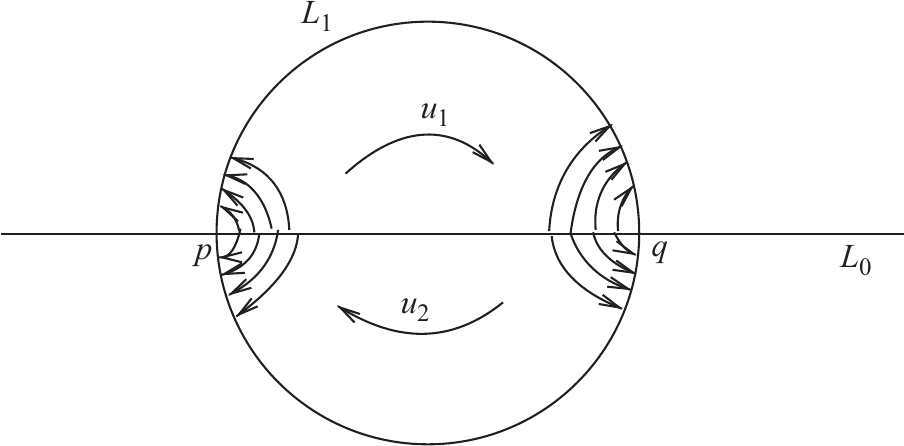
\includegraphics[width=.62\textwidth]{chapters/ch16-monotone-lagrangian-floer/figures/figure-16-1.png}
 \caption{全纯映射 $u_1,u_2$。}
 \label{fig:holomorphic-maps-u1-u2}
\end{figure}

由带边界的\personRiemann{}映射定理的简单应用可知，$\mathcal M(p,q;B_1)$ 恰有一个元素，
它由 $u_1:\mathbb R\times[0,1]\to\mathbb C$ 代表，其像为显然的上半圆盘（图
\ref{fig:holomorphic-maps-u1-u2}）。类似地，$\mathcal M(q,p;B_2)$ 恰有一个元素，
其像为下半圆盘。再对\personRiemann{}--\personHilbert{}问题作简单线性分析，还可证明这些映射正则，
即其线性化映射满射。由维数考察得到
\[
 \partial([\ell_p,w])=[q,w\#B_1],
 \qquad
 \partial([\ell_q,w'])=[p,w'\#B_2],
\]
其中 $w,w'$ 分别遍历 $\ell_p,\ell_q$ 的\termBoundingDisc{}。
\end{example}

\begin{exercise}
\label{ex:prove-plane-boundary-formula}
证明上述断言。
\end{exercise}

现在分析 $\mathcal M(p,p;B)$。把 $\mathcal M(p,p;B)$ 的每个元素视为对应于
$\widetilde{\mathcal M}(p,p;B)$ 中元素的无参数化曲线，由\personRiemann{}映射定理可证，
它由 $-1<\ell<1$ 时的全纯映射 $u_\ell:\mathbb R\times[0,1]\to\mathbb C$
组成，并满足
\[
 \begin{gathered}
 u_\ell(\mathbb R\times\{0\})\subset\mathbb R\times\{0\},\qquad
 u_\ell(\mathbb R\times\{1\})\subset\partial D^2,\qquad [u_\ell]=B,\\
 u_\ell(-\infty,\cdot)=u_\ell(\infty,\cdot)=\ell_p,\qquad
 u_\ell(0,0)=(\ell,0).
 \end{gathered}
\]
由对称性，$u_\ell$ 还必满足 $u_\ell(0,1)=(1,0)$。可以证明，上述族确实给出
$\mathcal M(p,p;B)$ 的全部元素，并且所有映射都是\personFredholm{}正则的。由此描述，
$\mathcal M(p,p;B)$ 的一个自然紧化是在 $\ell\to1$ 的一端添入断裂流线
$u_1\#u_2$，并添入 $\ell\to-1$ 时的另一端。

\begin{figure}[htbp]
 \centering
 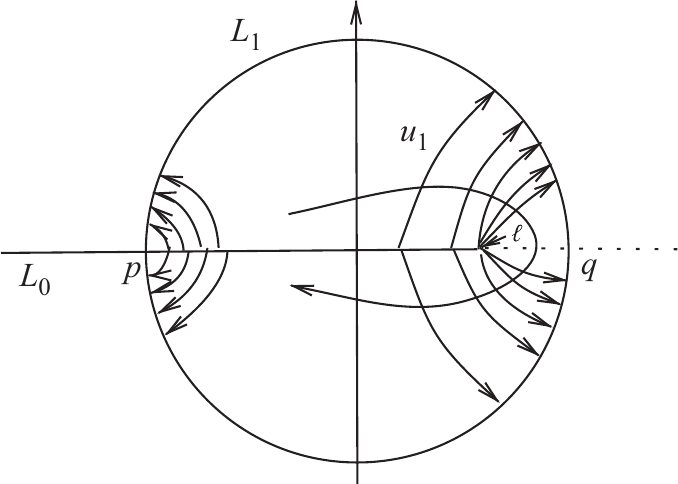
\includegraphics[width=.58\textwidth]{chapters/ch16-monotone-lagrangian-floer/figures/figure-16-2.png}
 \caption{全纯映射 $u_\ell$。}
 \label{fig:holomorphic-maps-ul}
\end{figure}

见图\ref{fig:holomorphic-maps-ul}。注意 $u_\ell$ 满足：
\begin{enumerate}[label=(\arabic*)]
\item $u_\ell(\mathbb R\times\{0\})\subset\{(t,0)\mid-1<t\leq\ell\}$；特别地，
当 $\ell\to-1$ 时，$u_\ell|_{\mathbb R\times\{0\}}$ 收敛到常值映射 $(-1,0)$；
\item $u_\ell|_{\mathbb R\times\{1\}}$ 的像恰好绕边界 $\partial D^2$ 一周。
\end{enumerate}
还可以验证，对任意紧子集
$K\subset\mathbb R\times[0,1]\setminus\{(0,1)\}$，
\[
 \|du_\ell\|_{\infty,K}\longrightarrow0\quad(\ell\to-1),
\]
同时还有
\[
 |du_\ell(0,1)|\nearrow\infty.
\]

由此分析可知，当 $\ell\to-1$ 时，上图背后的真实情形是出现了与如下奇异曲线
对应的\emph{稳定}流线：
\[
 (u_\infty,\mathbb R\times[0,1],\{(0,1)\})
 \cup(w,D^2,\{\mathrm{pt}\}).
\]
这里 $(u_\infty,\mathbb R\times[0,1],(0,1))$ 是主分支，
$u_\infty:\mathbb R\times[0,1]\to\mathbb C$ 是取常值
$p=(-1,0)$ 的映射，其定义域满足
\[
 (\mathbb R\times[0,1],\{(0,1)\})
 \cong(D^2\setminus\{\pm1\},\{\sqrt{-1}\}),
\]
而 $w:(D^2,\partial D^2)\to(\mathbb C,L_1)$ 是显然的包含映射，其定义域为边界
$\partial D^2$ 上带一个标记点的圆盘 $D^2$。

这个位形是一条可容许的稳定流线：$u_\infty$ 的定义域在边界上有三个特殊点，故它
稳定；$w$ 是非常值映射，故也稳定，因而两个映射的自同构群都平凡。对
$\mathcal M(p,p;B)$ 的上述分析计算出矩阵元
\[
 \bigl\langle(\partial\circ\partial)([\ell_p,w]),[\ell_p,w\#B]\bigr\rangle=1
\]
以及
\[
 \bigl\langle(\partial\circ\partial)([\ell_p,w]),[\ell_p,w\#B']\bigr\rangle=0
\]
（对任意 $B'\in\pi_2(p,p)$ 且 $B'\neq B$）。这清楚表明
$\partial\circ\partial\neq0$。

这个例子说明，当 $\mu(B)=2$ 时，$\mathcal M(p,p;B)$ 的边界可以含有并非断裂流线
类型的分支。还要注意，\emph{上述圆盘 $w$ 的马斯洛夫指标为 $2$}；稍后我们将看到，这并非
巧合。

事实上，对无边界紧\personRiemann{}曲面中的嵌入拉格朗日子流形而言，上述障碍是定义\personFloer{}同调的唯一障碍。在曲面上，每个一维子流形都是拉格朗日的，故紧嵌入拉格朗日子流形
是嵌入圆周的有限不交并。下面的曲面一般定理概括了这一讨论。

\begin{theorem}
\label{thm:surface-unobstructed-floer}
设 $\Sigma$ 是带面积形式的定向紧曲面。以 $\mathcal E_\Sigma^{\mathrm{ad}}$ 表示所有
连通分支都非零伦的嵌入拉格朗日子流形之集合。则对任意
$L_1,L_2\in\mathcal E_\Sigma^{\mathrm{ad}}$，取适当的\personNovikov{}环后，\personFloer{}同调
$HF(L_1,L_2;\Lambda)$ 有良定义。
\end{theorem}

在此意义下给出如下定义。

\stfhSubIndex{I189}{Wuzhangai}{无障碍（unobstructed）}{Qianruquxiandewuzhangaixing}{嵌入曲线的无障碍性（of embedded curves）}
\begin{definition}
\label{def:unobstructed-curve-surface}
设 $\Sigma$ 是带面积形式的定向紧曲面。若嵌入曲线 $\gamma\subset\Sigma$（不必连通）
没有零伦的连通分支，则称它是\termUnobstructed{}的。
\end{definition}

这是 (FOOO09) 所引入定义在二维曲面上的拉格朗日子流形情形之特例。关于高亏格曲面\termFukayaCategory{}的详细研究，可参见 (Ab08)；其中\personAbouzaid{}计算了 $\Sigma$ 上导出\personFukaya{}范畴的\personGrothendieck{}群。

\section{单调拉格朗日子流形的例子}
\label{sec:examples-monotone-lagrangians}

如二维例子所示，一般拉格朗日子流形对子 $(L_0,L_1)$ 的\personFloer{}同调会遇到障碍。
对这一障碍及其形变理论的完整研究需要超出本书层次的数学；(FOOO09) 已对此作了
彻底处理，有意了解细节的读者可参阅该书。

\personFloer{}在 (Fl89b) 中引入单调辛流形的概念，以克服其研究哈密顿\personFloer{}同调时遇到的
横截性困难。

\begin{remark}
\label{rem:general-perturbation-transversality}
在一般构造\personGromov{}--\personWitten{}不变量所涉及的模问题中，利用殆复结构以外的扰动研究
横截性的一般途径，最早由\personKontsevich{}在其著名论文 (Kon95) 中提出。

\stfhIndex{I117}{Cangxijiegou}{仓西结构（Kuranishi structure）}
\stfhIndex{I155}{Duozhongzhedietujing}{多重折叠途径（polyfold approach）}
如今，这种一般扰动横截性理论本质上有两种不同途径：一种是\emph{有限维壳上}途径，另一种
是\emph{无穷维离壳}途径。前一种是\personFukaya{}与\personOno{} (FOn99) 所采用的\termKuranishiStructure{}与多截面
方法，它是求解非线性方程的经典\personLyapunov{}约化方法之加强形式（相关构造亦见
(LT98)）；代数几何学家在 (LiT98)、(Be97)、(BF97) 中也采用这一途径。后一种途径
由\personBerndSiebert{} (Sie99) 采用，较近则以\personHofer{}、\personKrzysztofWysocki{}与\personZehnder{}的\termPolyfold{}途径
(HWZ07)、(H08) 为代表，尝试在离壳设置中对原方程作整体扰动（相关构造亦见
(Ru99)）。

即使 (FOn99) 问世二十年之后，这个横截性问题仍然是一个即便在辛几何专家之间也
需要进一步澄清的问题。
\end{remark}

受\personFloer{}对单调辛流形研究的启发，作者在 (Oh93a) 中挑出了单调拉格朗日子流形这一
类，以便把\personFloer{}对对子 $(L_0,L_1)$ 的同调理论构造推广到正合情形之外。这类拉格朗日
子流形避开了开\personRiemann{}曲面（亏格为零）的紧化模空间所涉及的大部分复杂横截性问题，
并使人能够无缝推广\personFloer{}的定义，依定义 16.1.1 中\personFloer{}原来的定义来定义映射
$\partial:CF(L_0,L_1)\to CF(L_0,L_1)$。

然而，(Oh93a) 已经注意到、(Oh95a) 后来又进一步强调，即使在这一良好情形中，也可能
出现\termAnomaly{}，即
\begin{equation}
 \partial^2\neq0,
\label{eq:monotone-boundary-anomaly}
\end{equation}
除非对子 $(L_0,L_1)$ 满足某个与马斯洛夫指标为 $2$ 的全纯圆盘之几何密切相关的
相容性条件。

\begin{remark}
\label{rem:role-of-monotonicity}
从内蕴辛拓扑的观点看，单调性既不自然也不灵活，因此它在一般辛拓扑中的作用对作者
而言尚未完全清楚。不过，它足以丰富地展示全纯圆盘如何在\personFloer{}同调中产生\emph{\termAnomaly{}}与
\emph{障碍}，并在\emph{非正合}背景下检验各种\personFloer{}理论构造。以某种方式处理上述障碍后，它也
自然推广了曲面上拉格朗日子流形\personFloer{}同调的讨论。在尝试借助障碍--形变理论与\termKuranishiStructure{}技术，把各种代数和几何结构完整实现于一般拉格朗日子流形的背景中
之前，单调情形是一个很好的试验场。近来，与（几乎）环面流形及镜像对称相关的许多
有趣单调拉格朗日环面例子已被发现；见 (FOOO12a)、(Wu12)、(Via13, Via14)。
\end{remark}

下面给出单个拉格朗日子流形版本的 $G(L_0,L_1;\ell_0)$；它也类似于环境辛流形
$(M,\omega)$ 的群
\[
 \Gamma_\omega=\Gamma(M,\omega)
 =\frac{\pi_2(M)}{\ker\omega\cap\ker c_1}.
\]
以 $I_\omega:\pi_2(M,L)\to\mathbb R$ 表示辛面积的取值。另定义整值同态
$I_\mu:\pi_2(M,L)\to\mathbb Z$：
\[
 I_\mu(\beta)=\mu\bigl(w^*TM,(\partial w)^*TL\bigr),
\]
其中右端是丛对
\[
 (w^*TM,(\partial w)^*TL)
\]
的马斯洛夫指标，而 $w:(D^2,\partial D^2)\to(M,L)$ 是 $\beta$ 的一个（因而
任意一个）代表。

\begin{definition}
\label{def:lagrangian-novikov-group}
定义
\[
 G(L;\omega)=\frac{\pi_2(M,L)}{\ker I_\omega\cap\ker I_\mu},
\]
并把 $\Lambda_{(L;\omega)}$ 定义为相应的\personNovikov{}环。
\end{definition}

简要回顾\personNovikov{}环 $\Lambda_{(\omega,L)}(R)$ 及其子环
$\Lambda_{0,(\omega,L)}(R)$ 的基本性质，其中 $R$ 是交换环，例如可取
$\mathbb Z_2$、$\mathbb Z$ 或 $\mathbb Q$。令
\[
 q^\beta=T^{\omega(\beta)}e^{\mu_L(\beta)},
\]
并令
\[
 \deg(q^\beta)=\mu_L(\beta),\qquad E(q^\beta)=\omega(\beta),
\]
于是 $\Lambda_{(\omega,L)}$ 与 $\Lambda_{0,(\omega,L)}$ 一般成为分次环。典范赋值
$\nu:\Lambda_{(\omega,L)}\to\mathbb R$ 定义为
\[
 \nu\left(\sum_\beta a_\beta T^{\omega(\beta)}e^{\mu_L(\beta)}\right)
 =\min\{\omega(\beta)\mid a_\beta\neq0\}.
\]
它诱导子环 $\Lambda_{0,(\omega,L)}\subset\Lambda_{(\omega,L)}$ 上的赋值，并进而
诱导其上的自然滤过。这使 $\Lambda_{(\omega,L)}$ 成为滤过分次环。对一般拉格朗日
子流形，该环甚至不必是\personNoether{}环。

下面定义单调拉格朗日子流形。

\stfhIndex{I131}{JixiaoMasiluofushu}{极小马斯洛夫数（minimal Maslov number）}
\stfhSubIndex{I133}{Dandiaolagelangriziliuxing}{单调拉格朗日子流形（monotone Lagrangian submanifold）}{Dingyi}{定义（definition）}
\begin{definition}
\label{def:monotone-lagrangian}
若紧拉格朗日子流形 $L\subset(M,\omega)$ 满足
\[
 I_\omega=\lambda I_\mu\qquad\text{对某个 }\lambda\geq0,
\]
则称 $L$ 是单调的。定义\emph{\termMinimalMaslovNumber{}} $\Sigma_L$ 为
$\operatorname{Im}I_\mu$ 的正生成元。
\end{definition}

\begin{exercise}
\label{ex:monotone-lagrangian-ambient}
证明单调拉格朗日子流形只存在于单调辛流形上。
\end{exercise}

\stfhIndex{I196}{Ruozhenghe}{弱正合（weakly exact）}
注意，所谓弱正合情形，即 $I_\omega=0$ 的情形，平凡地包含在上述情形中。若忽略
分次问题，则它可以完全按照正合情形 $\pi_2(M,L)=\{0\}$ 来研究。因此，本小节讨论
中假设 $L\subset M$ 单调、$\lambda>0$ 且 $I_\mu\neq0$。

下面的命题展示了这类拉格朗日子流形相对于一般拉格朗日子流形所具有的某些特殊辛
拓扑性质。

\begin{proposition}
\label{prop:monotone-lagrangian-group-rank-one}
设 $L\subset(M,\omega)$ 是单调拉格朗日子流形。则 $G(L;M,\omega)$ 是秩为 $1$
的自由\personAbel{}群，而 $\Lambda_{0,(\omega,L)}$ 成为一个离散赋值环，其剩余域是
$\Lambda_{(\omega,L)}$。
\footnote{译者注：原书此前把该群定义为 $G(L;\omega)$，本命题改写为
$G(L;M,\omega)$；且把 $\Lambda_{(\omega,L)}$ 称作
$\Lambda_{0,(\omega,L)}$ 的“剩余域”。译文照录，留待统一裁决。}
\end{proposition}

\stfhIndex{I056}{Kelifudehuanmian}{克利福德环面（Clifford torus）}
$\mathbb{RP}^n\subset\mathbb{CP}^n$ 以及例 5.19 中的\personClifford{}环面，都是单调
拉格朗日子流形的例子。

\begin{proposition}
\label{prop:clifford-torus-monotone}
考虑\personClifford{}环面 $T^n\subset\mathbb P^n$：
\[
 T^n=\{[z_0:z_1:\cdots:z_n]\in\mathbb P^n\mid |z_i|=1\}.
\]
该环面单调，其相伴群 $G(T^n;\mathbb P^n)$ 同构于 $\mathbb Z$。
\end{proposition}

\begin{proof}
容易验证
\[
 \pi_2(\mathbb P^n,T^n)\cong\pi_1(T^n)\oplus\pi_2(\mathbb P^n).
\]
若以 $\beta_i$ 表示圆盘
\[
 D_i=\{[z_0:z_1:\cdots:z_n]\in\mathbb P^n
 \mid z_j\equiv e^{\sqrt{-1}\theta_i^0}\text{ 对 }j\neq i\text{ 固定}\}
\]
之类，则在 $\pi_2(\mathbb P^n,T^n)$ 中有关系
\[
 \beta_0+\cdots+\beta_n=\alpha,
\]
其中 $\alpha$ 是 $\pi_2(\mathbb P^n)$ 的（正）生成元。又有
\begin{equation}
\begin{aligned}
 \mu(\beta_i)&=2=\frac{c_1(\alpha)}{n+1},\\
 \omega(\beta_i)&=\frac{\omega(\alpha)}{n+1}=2\pi.
 \end{aligned}
\label{eq:clifford-torus-monotonicity}
\end{equation}
\footnote{译者注：对 $\mathbb P^n$ 的标准正生成元通常有
$c_1(\alpha)=n+1$，故原书所印 $2=c_1(\alpha)/(n+1)$ 与此不相容；译文照录。}
这就证明了单调性。

此外，\eqref{eq:clifford-torus-monotonicity} 还蕴含所有 $\beta_i$ 在
$G(T^n;\mathbb P^n)$ 中定义同一个元素，记为 $\beta$，且
$\alpha=(n+1)\beta$。因此
\[
 G(T^n;\mathbb P^n)=\mathbb Z\cdot[\beta]\cong\mathbb Z.
\]
\end{proof}

再考虑其他标准环面
\[
 T_{(c_0,\ldots,c_n)}
 =\{[z_0:\cdots:z_n]\in\mathbb P^n\mid |z_i|=c_i>0\}.
\]
它们并不单调。以 $\beta_i$ 和 $\alpha$ 表示与上述
$c_0=\cdots=c_n$ 情形类似定义的类。依赖于数集
\[
 \{\omega(\beta_0),\ldots,\omega(\beta_n),\omega(\alpha)=2\pi\}
\]
的有理相关性，$G(T_{(c_0,\ldots,c_n)};\mathbb P^n)$ 的秩在 $1$ 与 $n+1$
之间变化。该例可进一步推广到环面流形的拉格朗日环面纤维；(CO06)、
(FOOO10b, FOOO11a) 对此作了细致分析。

单调性条件主要是为寻找一个条件而设计的，使 (Oh93a) 所定义的朴素\personFloer{}同调能够
构造。不过，第 3.7.2 节所述拉格朗日悬挂构造保持这一条件。

\begin{proposition}
\label{prop:monotone-suspension}
设 $L\subset(M,\omega)$ 是任意紧单调拉格朗日嵌入，$(h,\psi)$ 是第 3.7.2 节
意义下它的正合拉格朗日圈。则相伴悬挂
\[
 \iota_{(h,\psi)}:S^1\times L\longrightarrow T^*S^1\times M
\]
关于 $T^*S^1\times M$ 上的直和辛形式 $\omega_0\oplus w$ 是具有相同\termMonotonicityConstant{}的
单调拉格朗日嵌入。
\footnote{译者注：原书此处的直和辛形式印作 $\omega_0\oplus w$，而环境辛形式一直
记作 $\omega$；译文照录。}
\end{proposition}

\begin{exercise}
\label{ex:prove-monotone-suspension}
证明该命题。
\end{exercise}

还从命题 3.7.7 回忆，$\iota_{(h,\psi)}$ 在 $T^*S^1\times M$ 中哈密顿同痕于乘积
嵌入 $o_{S^1}\times L$。

\stfhIndex{I154}{Boerjieluoweiqi}{波尔捷罗维奇（Polterovich）}
\personPolterovich{}在研究 $\Ham(S^2)$ 的\personHofer{}直径时利用了上述命题，并把拉格朗日\personFloer{}同调的\personKunneth{}公式的一个版本应用于 $S^2$ 的赤道，巧妙地证明了下面的定理。第
17.6 节将依原论文 (Po98b) 给出证明。

\begin{theorem}[\personPolterovich{}]
\label{thm:hofer-diameter-s2-infinite}
$\Ham(S^2)$ 的\personHofer{}直径为无穷。
\end{theorem}

下面说明第 3.7.3 节所述\personChekanov{}环面 (Che96b) 的一个变体。

\begin{example}[在 $S^2\times S^2$ 中的\personChekanov{}环面]
\label{ex:chekanov-torus-s2xs2}
\personChekanov{}的环面最初通过把第 3.7.3 节所述悬挂构造用于标准圆周
$S^1\subset\mathbb C$ 而在 $\mathbb C^2$ 中构造（见例 16.3.6(3)）。适当选择\personChekanov{}悬挂中出现的参数，可将该环面嵌入 $S^2\times S^2$，成为一个奇异单调
拉格朗日环面：它与乘积
$S^1_{\mathrm{eq}}\times S^1_{\mathrm{eq}}\subset S^2\times S^2$ 不哈密顿同痕
（证明见 (EP10)、(FOOO12a)）。其构造可描述如下（此描述见 (AF08)）。把
$S^2\times S^2\setminus\overline\Delta$ 等同于单位圆盘丛 $D^1(TS^2)$。
(AF08) 中研究的拉格朗日环面，是 $\partial D^r(TS^2)$ 上经过一个给定点（比如北极
$N$）的简单闭定向测地线之并。适当选取 $r>0$，可以证明该环面在
$S^2\times S^2\supset D^1(TS^2)$ 中单调。把它记作 $T(r)$。
\end{example}

\begin{exercise}
\label{ex:unique-monotone-chekanov-radius}
证明上述例子中恰有一个 $0<r<1$ 的选择使环面 $T(r)$ 单调，并求出 $r$。
\end{exercise}

\personChekanov{}与\personSchlenk{} (CS10) 在辛向量空间或复射影空间中构造了许多单调拉格朗日环面，
并研究了其中哪些例子彼此不同。

\stfhIndex{I146}{Dandiankaigeluomofu-Weitengbubianliang}{单点开格罗莫夫--威腾不变量（one-point open Gromov--Witten invariant）}
\section{\termOnePointOpenGromovWittenInvariant{}}
\label{sec:one-point-open-gw-invariant}

单调拉格朗日子流形的一个良好性质，是不存在第 10.6 节所述的\emph{负多重覆叠问题}。
这是因为每个非常值伪全纯圆盘都具有正马斯洛夫指标。由此可以定义不依赖于相容殆复
结构选择的\emph{开\personGromov{}--\personWitten{}不变量}。

本节依照 (Oh95a) 的说明，构造这一\emph{单点不变量}并证明其辛不变性。

对相容殆复结构 $J_0$，定义
\[
 \widetilde{\mathcal M}(L;\beta;J_0)
 =\{w:(D^2,\partial D^2)\to(M,L)\mid
 \overline\partial_Jw=0,\ w(\partial D^2)\subset L,\ [w]=\beta\}
\]
及其商
\[
 \mathcal M(L;\beta;J_0)
 =\widetilde{\mathcal M}(L;\beta;J_0)/PSL(2,\mathbb R).
\]
回忆指标公式
\begin{equation}
 \operatorname{vir.dim}\widetilde{\mathcal M}(L;\beta;J_0)
 =n+\mu_L(\beta),
\label{eq:disc-moduli-virtual-dimension}
\end{equation}
其中 $\mu_L(\beta)$ 是丛对 $(w^*TM,(\partial w)^*L)$ 的马斯洛夫指标
$\mu(w^*TM,(\partial w)^*L)$，而 $w$ 是
$\widetilde{\mathcal M}(L;\beta;J_0)$ 的某个（因而任意一个）元素。
\footnote{译者注：原书两次把边界丛写作 $(\partial w)^*L$，而非通常的
$(\partial w)^*TL$；译文照录。}
我们还考察带一个标记点的 $J_0$-全纯圆盘模空间
$\mathcal M_1(L;\beta;J_0)$。

给定光滑道路 $J:[0,1]\to\mathcal J_\omega$，定义参数化模空间
\[
 \mathcal M^{\mathrm{para}}(L;\beta;J)
 =\coprod_{t\in[0,1]}\{t\}\times\mathcal M(L;\beta;J(t)),
\]
\[
 \mathcal M_1^{\mathrm{para}}(L;\beta;J)
 =\coprod_{t\in[0,1]}\{t\}\times\mathcal M_1(L;\beta;J(t)),
\]
把它们看作 $[0,1]$ 上的纤维化。下面给出紧性结果。

\begin{proposition}
\label{prop:minimal-maslov-two-disc-compactness}
设 $L\subset(M,\omega)$ 单调，其\termMinimalMaslovNumber{} $\Sigma_L\geq2$。
设 $\beta\in\pi_2(M,L)$ 满足 $\mu(\beta)=2$。则：
\begin{enumerate}[label=(\arabic*)]
\item 对任意相容殆复结构 $J_0$，$\mathcal M(L;\beta;J_0)$ 与
$\mathcal M_1(L;\beta;J_0)$ 都紧；
\item 对道路 $J:[0,1]\to\mathcal J_\omega$，参数化模空间
$\mathcal M^{\mathrm{para}}(L;\beta;J)$ 与
$\mathcal M_1^{\mathrm{para}}(L;\beta;J)$ 都紧。
\end{enumerate}
\end{proposition}

\begin{proof}
这是开情形稳定映射紧性定理的直接推论。这里只证明第一条。设
$w_i\in\widetilde{\mathcal M}(L;\beta;J_0)$ 是一个序列。需要证明 $w_i$ 有一个
子序列，在模去 $PSL(2,\mathbb R)$ 作用后收敛到稳定映射。

由于 $[w_i]=\beta$ 固定，
\[
 E_{J_0}(w_i)=\int w_i^*\omega=\omega(\beta),
\]
故序列 $w_i$ 具有一致能量上界。稳定映射紧性定理于是说明，可以选取一个仍记作
$w_i$ 的子序列，收敛到稳定映射
\[
 w_\infty=\sum_{\ell=1}^{N}v_\ell,
\]
其中每个 $v_\ell$ 或为 $J_0$-全纯圆盘，或为 $J_0$-全纯球面。若 $v_\ell$ 是球面，
以 $\mu(v_\ell)$ 表示 $2c_1(v_\ell)$；若它是边界落在 $L$ 上的圆盘，则以
$\mu(v_\ell)$ 表示其马斯洛夫指标。

由于 $\mu(\beta)=2$ 极小，且
\[
 2=\mu(w_\infty)=\sum_{\ell=1}^{N}\mu(v_\ell),
\]
单调性蕴含上述和中至多有一个非常值分支。另一方面，$w_\infty$ 的稳定性又蕴含其中
不能有常值分支。因此必有 $N=1$，从而 $w_i$ 经适当重参数化后确实收敛。

类似论证证明 $\mathcal M_1(L;\beta;J_0)$ 及参数化空间的紧性。
\end{proof}

下面回忆通过扰动殆复结构得到的横截性结果。设 $L\subset(M,\omega)$ 是任意紧单调
拉格朗日子流形，以
\[
 \widetilde{\mathcal M}^{\mathrm{inj}}(L;\beta;J_0)
 \subset\widetilde{\mathcal M}(L;\beta;J_0)
\]
表示由\termSomewhereInjective{}的 $J_0$-全纯圆盘组成的子集。

闭曲面情形的如下基本横截性结果已在第 10.4、10.5 节证明。

\begin{proposition}
\label{prop:disc-evaluation-transversality}
设 $x\in L$。存在稠密子集
$\mathcal J_\omega(L,x)\subset\mathcal J_\omega$，使对所有
$\beta\in\pi_2(M,L)$：
\begin{enumerate}[label=(\arabic*)]
\item $\widetilde{\mathcal M}^{\mathrm{inj}}(L;\beta;J_0)$ 横截；
\item $\operatorname{ev}_\beta:\mathcal M_1^{\mathrm{inj}}(L,\beta;J_0)\to L$
横截于 $x$。
\end{enumerate}
对 $J=\{J(t)\}_{0\leq t\leq1}$ 的参数化模空间，同样结论成立。
\end{proposition}

称这样的对子 $(J_0,x_0)$ 为\termTransversePair{}。对\termTransversePair{} $(J_0,x_0)$，命题
\ref{prop:minimal-maslov-two-disc-compactness} 与
\ref{prop:disc-evaluation-transversality} 蕴含：对任意满足 $\mu(\beta)=2$ 的
$\beta$，$\operatorname{ev}_\beta^{-1}(x_0)$ 是紧零维流形（若非空）。

\begin{lemma}
\label{lem:minimal-maslov-discs-somewhere-injective}
设 $J_0$ 是任意相容殆复结构，不必正则。设 $L\subset(M,\omega)$ 单调且
$\Sigma_L>0$，并取满足 $\mu(\beta)=\Sigma_L$ 的
$\beta\in\pi_2(M,L)$。则
\[
 \widetilde{\mathcal M}^{\mathrm{inj}}(L;\beta;J_0)
 =\widetilde{\mathcal M}(L;\beta;J_0),
\]
即对任意 $J_0\in\mathcal J_\omega$，
$\widetilde{\mathcal M}(L;\beta;J_0)$ 中所有 $J_0$-全纯圆盘都\termSomewhereInjective{}。特别地，命题\ref{prop:disc-evaluation-transversality} 对完整
模空间成立。
\end{lemma}

\begin{proof}
第一条来自\termMinimalMaslovNumber{} $\Sigma_L$ 的定义：由像的结构定理——球面情形的
定理 8.7.3，以及圆盘情形的 (Laz00)、(KO00)——无论 $J_0$ 正则与否，每个
$J_0$-全纯圆盘都必为单圆盘。第二条则由单调性假设与 $\mu(\beta)=\Sigma_L$ 立即
推出，因为它们排除了冒泡。
\end{proof}

记
\[
 \Phi_{J_0}(L;x_0)
 =\sum_{\beta:\,\mu(\beta)=2}\#\bigl(\operatorname{ev}_\beta^{-1}(x_0)\bigr).
\]
\emph{从此以后不再特别说明：对一般 $L$，计数取 $\mathbb Z_2$-系数；当拉格朗日子流形
$L$（相对）spin 时，使用 $\mathbb Z$-系数。}

\begin{lemma}
\label{lem:one-point-count-invariance}
设 $L\subset(M,\omega)$ 单调且 $\Sigma_L\geq2$。设 $(J_0,x_0)$ 与
$(J_1,x_1)$ 是\termTransversePair{}，并且 $[x_0]=[x_1]\in\pi_0(L)$。则
\[
 \Phi_{J_0}(L;x_0)=\Phi_{J_1}(L;x_1).
\]
\end{lemma}

\begin{proof}
固定嵌入道路 $\gamma:[0,1]\to L$，其中 $\gamma(0)=x_0$、$\gamma(1)=x_1$。
由评价横截性的参数化版本及横截性延拓定理，可选道路
$J:[0,1]\to\mathcal J_\omega$，使得对所有 $\mu(\beta)=2$ 的 $\beta$，
$\widetilde{\mathcal M}^{\mathrm{para}}(L;\beta;J)$ 横截，且评价映射
\[
 \begin{aligned}
 \operatorname{Ev}_\beta:
 \mathcal M_1^{\mathrm{para}}(L;\beta;J)&\longrightarrow[0,1]\times L,\\
 (t,(w,z))&\longmapsto(t,w(z))
 \end{aligned}
\]
横截于 $\Lambda=\operatorname{id}\times\gamma:[0,1]\to[0,1]\times L$。指标公式给出
\[
 \dim\mathcal M_1^{\mathrm{para}}(L;\beta;J)=n+1,
\]
故 $\operatorname{Ev}_\beta^{-1}(\Lambda)$ 是紧一维流形，其边界为
\[
 \{0\}\times\operatorname{ev}_\beta^{-1}(x_0)
 \coprod
 \{1\}\times\operatorname{ev}_\beta^{-1}(x_1).
\]
由紧一维流形的分类定理，
\[
 \#\bigl(\operatorname{ev}_\beta^{-1}(x_0)\bigr)
 =\#\bigl(\operatorname{ev}_\beta^{-1}(x_1)\bigr).
\]
依定义即得结论。
\end{proof}

由此可以如下定义单点 GW 不变量。

\begin{definition}
\label{def:one-point-open-gw-invariant}
设 $L\subset(M,\omega)$ 是紧单调拉格朗日子流形，$\Sigma_L\geq2$；以
$\pi\in\pi_0(L)$ 表示 $L$ 的一个连通分支。相对于 $\pi$ 的单点 GW 不变量定义为
\[
 \Phi(L;\pi)=\Phi_{J_0}(L;x_0),
\]
其中 $(J_0,x_0)$ 是满足 $[x_0]=\pi\in\pi_0(L)$ 的\termTransversePair{}。当 $L$ 连通时，简记
\[
 \Phi(L;\{\mathrm{pt}\})=\Phi_{J_0}(L;x_0),
\]
称其为 $L\subset(M,\omega)$ 的单点 GW 不变量。
\end{definition}

下面考察几个例子。

\begin{example}
\label{ex:one-point-open-gw-examples}
\begin{enumerate}[label=(\arabic*)]
\item \stfhPropertyLabel{（标准环面）} 考虑标准环面
\[
 T^n=\underbrace{S^1(1)\times\cdots\times S^1(1)}_{n\text{ 个}}
 \subset\mathbb C^n\cong\mathbb R^{2n}.
\]
有 $\pi_2(\mathbb C^n,T^n)\cong\pi_1(T^n)\cong\mathbb Z^n$。以
$\beta_i$（$i=1,\ldots,n$）表示由映射
\[
 \begin{aligned}
 w_i:(D^2,\partial D^2)&\longrightarrow(\mathbb C^n,T^n),\\
 w_i(z)&=(1,\ldots,\underbrace{z}_{i\text{th}},\ldots,1)
 \end{aligned}
\]
代表的 $\pi_2(\mathbb C^n,T^n)$ 的显然生成元。计算其马斯洛夫指标与辛面积可知，
该环面单调，\termMonotonicityConstant{}为 $\lambda=\pi$。这些映射显然是经过点
$x_0=(1,\ldots,1)$ 的全纯映射，故至少有 $n$ 个彼此不同、马斯洛夫指标为 $2$
的全纯圆盘。

\item \stfhPropertyLabel{（\personClifford{}环面）} 这次考虑\personClifford{}环面
$T^n\subset\mathbb{CP}^n$。它由 $\mathbb C^{n+1}$ 上乘积圆周作用的商
$T^{n+1}/S^1\subset S^{2n+1}/S^1\cong\mathbb{CP}^n$ 定义。在射影坐标中有全纯
圆盘
\[
 w_j:(D^2,\partial D^2)\to(\mathbb{CP}^n,T^n),
 \qquad z\longmapsto[1;\ldots;\underbrace{z}_{j\text{th}};\ldots;1]
\]
（$j=1,\ldots,n+1$）。把
$\Phi(T^n,\mathbb{CP}^n;\{\mathrm{pt}\})=n+1$ 的证明留作习题。

\item \stfhPropertyLabel{（\personChekanov{}环面）} 对标准圆周
$S^1(1)\subset\mathbb R^2\cong\mathbb C$ 施行\personChekanov{}悬挂，得到\personChekanov{}环面
\[
 \Theta_0(S^1(1))\subset\mathbb R^2,
 \qquad
 \Theta_0(S^1(1))=I_1(N_0\times S^1(1)).
\]
\footnote{译者注：原书把所得\personChekanov{}环面的环境写作 $\mathbb R^2$；但紧接着定义的
辛嵌入以 $T^*\mathbb R^2$ 为靶，维数提示这里可能有环境维数的排印问题。译文照录。}
这里 $N_0$ 是 $T^*S^1$ 的零截面，$I_1=(i_1^*)^{-1}$ 是辛嵌入
\[
 I_1=(i_1^*)^{-1}:T^*(\mathbb R\times S^1)\longrightarrow T^*\mathbb R^2,
\]
其中 $i_1:S^1\times\mathbb R\to\mathbb R^2$ 定义为
\[
 i_1(\theta,q)=(e^q\cos(2\pi\theta),e^q\sin(2\pi\theta)).
\]
\personEliashberg{}与\personPolterovich{}在 (EP97) 中证明
\[
 \Phi(\Theta_0(S^1(1));\{\mathrm{pt}\})=1.
\]
不久前，\personChekanov{}与\personSchlenk{}尝试对若干显式辛流形类上的单调拉格朗日子流形集合
作完整分类 (CS10)。
\end{enumerate}
\end{example}

\begin{exercise}
\label{ex:classify-minimal-maslov-discs-tori}
证明例\ref{ex:one-point-open-gw-examples} 中给出的 $\mathbb C^n$ 内标准环面及
$\mathbb{CP}^n$ 内\personClifford{}环面的圆盘全都横截，并且它们给出了经过环面中给定点
$x_0$ 的所有马斯洛夫指标为 $2$ 的全纯圆盘。（若计入这些圆盘的定向，则它们全都
正贡献，故
$\Phi(T^n,\mathbb C^n;\mathrm{pt})=n$ 且
$\Phi(T^n,\mathbb{CP}^n;\{\mathrm{pt}\})=n+1$。定向研究见第 15.4 节。）
\end{exercise}

\stfhIndex{I054}{Qiekanuofu}{切卡诺夫（Chekanov）}
上述单点不变量计算立即导出\personChekanov{}定理 (Che96b)。

\begin{theorem}[\personChekanov{}]
\label{thm:standard-chekanov-tori-not-symplectically-equivalent}
标准环面 $T^2=S^1(1)\times S^1(1)$ 与\personChekanov{}环面
$\Theta_0(S^1(1))$ 不辛等价。
\end{theorem}

\personChekanov{}最初通过考察\personEkeland{}--\personHofer{}容量序列的行为证明该定理。应指出，标准环面与\personChekanov{}环面都满足下列条件：
\begin{enumerate}[label=(\arabic*)]
\item \termMinimalMaslovNumber{}为 $2$；
\item \termMonotonicityConstant{}为 $\pi$；
\item 第一\personEkeland{}--\personHofer{}容量为 $2\pi$。
\end{enumerate}
因此，没有简单的经典方法区分标准环面与\personChekanov{}环面。

\section{\personFloer{}边界算子的\termAnomaly{}}
\label{sec:anomaly-floer-boundary-operator}

本节考察单调拉格朗日子流形对子 $(L_0,L_1)$ 的\personFloer{}边界之构造。特别地，我们分析
(13.9.28) 中低虚维数——即\personMaslov{}--\personViterbo{}指标为 $0,1,2$——的\personFloer{}模空间结构。
记
\[
 \widetilde{\mathcal M}([\ell_p,w],[\ell_q,w'])
\]
为光滑\personFloer{}流线的集合，即并集
\[
 \widetilde{\mathcal M}([\ell_p,w],[\ell_q,w'])
 :=\bigcup_{w\#B\simeq w'}\widetilde{\mathcal M}(p,q;B),
\]
其中 $\widetilde{\mathcal M}(p,q;B)$ 是先前定义的连接 $p,q\in L_0\cap L_1$、满足
$[u]=B\in\pi_2(p,q)$ 的光滑\personFloer{}流线集合。

\subsection{\personFloer{} \termPreBoundaryMap{}的定义}
\label{subsec:floer-pre-boundary-definition}

先注意，若\termMonotonicityConstant{}为正，且 $\beta$ 容许一个非常值伪全纯圆盘，则
$\mu(\beta)>0$。从如下引理开始。

\begin{lemma}
\label{lem:maslov-one-discs-avoid-finite-set}
设 $L$ 紧，$F\subset L$ 是任意有限子集。则存在
$\mathcal J_\omega$ 的稠密子集 $\mathcal J_L(F)$，使对任意
$J_0\in\mathcal J_L(F)$ 以及任意满足 $\mu(\beta)=1$ 的
$\beta\in\pi_2(L)$，评价链
\[
 \operatorname{ev}_\beta:\mathcal M_1(L,J_0;\beta)\longrightarrow L
\]
都不与 $F$ 相交。
\end{lemma}

\begin{proof}
由指标公式，
\[
 \dim\mathcal M_1(L,J_0;\beta)=n+\mu(\beta)+1-3=n-1<n.
\]
$F$ 是有限点集，特别是零维的。于是，基于评价横截性边界版本（定理 16.3.2）的
维数计算说明：通有地选择 $J_0$ 时，评价链
$\operatorname{ev}_\beta:\mathcal M_1(L,J_0;\beta)\to L$ 不与 $F$ 相交。以
$\mathcal J_L(F)$ 表示所有这种 $J_0$ 组成的子集。
\end{proof}

现在证明下述定理。

\begin{theorem}
\label{thm:low-index-monotone-floer-moduli}
设 $L_0,L_1$ 单调且\termMinimalMaslovNumber{}非零，并且
$J_i\in\mathcal J_{L_i}(L_0\cap L_1)$（$i=0,1$），其中
$\mathcal J_{L_i}(L_0\cap L_1)$ 如引理
\ref{lem:maslov-one-discs-avoid-finite-set}。则存在子集
$\mathfrak j^{\mathrm{reg}}_{(L_0,L_1)}(J_0,J_1)\subset\mathfrak j_\omega$，
使对任意 $J\in\mathfrak j^{\mathrm{reg}}_{(L_0,L_1)}(J_0,J_1)$，下列断言成立：
\begin{enumerate}[label=(\arabic*)]
\item 对所有 $p,q\in L_0\cap L_1$ 和满足 $\mu(p,q;B)<0$ 的
$B\in\pi_2(p,q)$，$\mathcal M(p,q;B;J)=\varnothing$；
\item 对所有 $p,q\in L_0\cap L_1$ 和满足 $\mu(p,q;B)=0$ 的
$B\in\pi_2(p,q)$，除非 $p=q$ 且 $B=0\in\pi_2(p,q)$，否则
$\mathcal M(p,q;B;J)=\varnothing$；
\item 对所有 $p,q\in L_0\cap L_1$ 和满足 $\mu(p,q;B)=1$ 的
$B\in\pi_2(p,q)$，$\mathcal M(p,q;B;J)$ 是紧的零维流形，因而为有限集。
\end{enumerate}
\end{theorem}

\begin{proof}
证明基于指标公式 (16.3.3)、命题 15.1.5 与 16.3.2 的维数计算及相交论证。

由引理 15.1.4，$\mathbb R$ 自由作用于任意非常值流线 $u$（证明见 (Oh97a)）。
特别地，对任意\personFredholm{}正则 $J$，只要
$\widetilde{\mathcal M}(p,q;B;J)\neq\varnothing$，并且 $p\neq q$，或 $p=q$ 但
$B\neq0$，就有
\[
 \dim\widetilde{\mathcal M}(p,q;B;J)\geq1.
\]
（当 $p=q$ 时，可把 $\pi_2(p,p)$ 的每个元素等同于 $\pi_2(L_0)$ 或
$\pi_2(L_1)$ 中的元素。）因此，对
$J\in\mathfrak j^{\mathrm{reg}}_{(L_0,L_1)}(J_0,J_1)$，(1)、(2) 立即成立。
\footnote{译者注：原书证明此处把上述正则集合印作
$\mathcal P^{\mathrm{reg}}_{(L_0,L_1)}(J_0,J_1)$，与定理陈述中的
$\mathfrak j^{\mathrm{reg}}_{(L_0,L_1)}(J_0,J_1)$ 不一致；译文依定理记号补正。}

当 $\mu(p,q;B)=1$ 时，对任意 $(L_0,L_1)$-正则 $J$，
$\mathcal M(p,q;B;J)$ 都是零维的。只需证明它紧。否则存在序列
$u_i\in\mathcal M(p,q;B;J)$，当 $i\to\infty$ 时发生分裂或冒泡。

若 $u_i$ 在极限处分裂为 $(u_{\infty,1},u_{\infty,2})$，其中
$u_{\infty,1}\in\mathcal M(p,r;B_1)$、
$u_{\infty,2}\in\mathcal M(r,q;B_2)$，则
\[
 1=\mu(p,r;B_1)+\mu(r,q;B_2).
\]
因此二者的指标分别为 $1,0$，次序任意。但 $\mu(r,q;B_2)=0$ 意味着
$\dim\widetilde{\mathcal M}(r,q;B_2)=0$，除非 $r=q$ 且 $B_2=0$，否则不可能。
此时 $u$ 必须是常值条带，而这又不可能：这种圆盘具有由 $\tau$-平移产生的连续
$\mathbb R$-自同构群，故在模空间的稳定映射紧化定义中，其定义域会被压缩。注意
$\mathbb R\times[0,1]$ 共形等价于带两个标记点的圆盘，而后者不是稳定曲线。因此
$\mathcal M(p,q;B;J)$ 不可能有分裂端。

若 $u_i$ 发生冒泡，单调性蕴含每个气泡都有正指标。因此，球面气泡的指标至少为
$2>1$，维数计算排除了这种冒泡。唯一剩余可能是形如 $(u_0,w)$ 的极限，其中
$u_0\in\mathcal M(p,q;B';J)$，$w$ 是 $(L_0,J_0)$ 或 $(L_1,J_1)$ 的非常值圆盘
气泡。此时
\[
 1=\mu(p,q;B')+\mu(w).
\]
单调性再次给出 $\mu(w)>0$，故必有 $\mu(w)=1$、$\mu(p,q;B')=0$。后一等式蕴含
$p=q$、$B'=0$，所以 $u_0$ 是常值流线 $u_0\equiv p$。\personGromov{}--\personFloer{}极限之像的
连通性于是蕴含 $w$ 经过 $p\in L_0\cap L_1$。然而，由
$J_i\in\mathcal J_{L_i}(L_0\cap L_1)$ 的选择，引理
\ref{lem:maslov-one-discs-avoid-finite-set} 也排除了这种情形。
\end{proof}

除紧性外，另一个重要问题是模空间
$\mathcal M([\ell_p,w],[\ell_q,w'];J)$ 上的相容定向。第 15.6 节（亦见
(FOOO09)）已证明：若对子 $(L_0,L_1)$ 相对 spin 并给定相对 spin 结构，则存在一种
典范方式在模空间族 $\mathcal M([\ell_p,w],[\ell_q,w'];J)$ 上赋予相容定向。因此，
当 $(L_0,L_1)$ 相对 spin 时，整数
\[
 n([\ell_p,w],[\ell_q,w'];J)
 =\#\mathcal M([\ell_p,w],[\ell_q,w'];J),
 \qquad
 \mu[\ell_q,w']=\mu([\ell_p,w])+1,
\]
\stfhIndex{I088}{Fuluoeryubianjieyingshe}{弗洛尔预边界映射（Floer pre-boundary map）}
有良定义。以它作为标准\personFloer{} \termPreBoundaryMap{}
\[
 \partial:CF_R^k(L_1,L_0;\ell_0)\longrightarrow CF_R^{k+1}(L_1,L_0;\ell_0)
\]
的矩阵元，定义
\[
 \partial([\ell_p,w])
 =\sum_{\mu(\ell_q,w')=\mu(\ell_p,w)+1}
 n([\ell_p,w],[\ell_q,w'])\cdot[\ell_q,w'].
\]
这里，当 $(L_0,L_1)$ 相对 spin 时 $R=\mathbb Z$，一般取 $R=\mathbb Z_2$。\personGromov{}--\personFloer{}紧性蕴含右端定义了 $CF_R^*(L_1,L_0;\ell_0)$ 中的元素，即满足\personNovikov{}有限性条件。因为\personFloer{}所定义的这个映射 $\partial$ 未必满足
$\partial^2=0$，所以称 $\partial$ 为\personFloer{} \termPreBoundaryMap{}。

\begin{figure}[htbp]
 \centering
 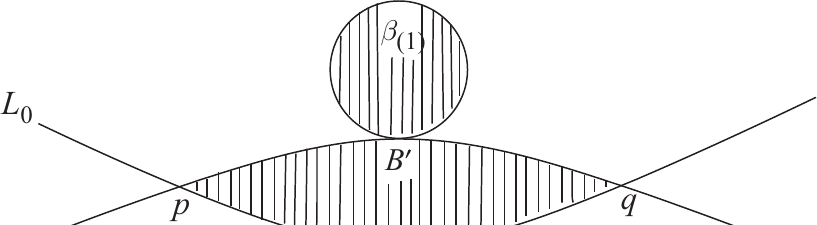
\includegraphics[width=.68\textwidth]{chapters/ch16-monotone-lagrangian-floer/figures/figure-16-3.png}
 \caption{余维 $1$ 的层 $\mathcal N(p,q;B';L_1,\beta_{(1)};J)$。}
 \label{fig:codimension-one-disc-bubble-stratum}
\end{figure}

\subsection{\termAnomaly{}与障碍}
\label{subsec:anomaly-and-obstruction}

现在研究\personFloer{} \termPreBoundaryMap{} $\partial$ 的边界性质。为此，需要分析虚维数为
$1$ 的模空间 $\mathcal M(p,q;B)$，并对每个这样的 $B$ 描述紧化模空间
$\overline{\mathcal M}(p,q;B)$ 中“余维 $1$”的奇异层。

考虑\personFloer{}流线模空间 $\widetilde{\mathcal M}(p,q;B';J)$ 及评价映射
\[
 \begin{aligned}
 \operatorname{ev}^{L_0}:\widetilde{\mathcal M}(p,q;B';J)&\to L_0,
 &(u,\tau)&\mapsto u(\tau,0),\\
 \operatorname{ev}^{L_1}:\widetilde{\mathcal M}(p,q;B';J)&\to L_1,
 &(u,\tau)&\mapsto u(\tau,1).
 \end{aligned}
\]
再考虑 $\mathcal M_1(L_0;\beta_{(0)};J_0)$、
$\mathcal M_1(L_1;\beta_{(1)};J_1)$ 及评价映射
\[
 \operatorname{ev}_0:\mathcal M_1(L_0;\beta_{(0)};J_0)\to L_0,
 \qquad
 \operatorname{ev}_1:\mathcal M_1(L_1;\beta_{(1)};J_1)\to L_1.
\]
下列集合描述 $\overline{\mathcal M}(p,q;B;J)$ 的余维 $1$ 层。

\begin{definition}
\label{def:disc-bubble-boundary-strata}
设 $p,q\in L_0\cap L_1$、$B'\in\pi_2(p,q)$，并且
$\beta_{(0)}\in G(L_0;\omega)$、$\beta_{(1)}\in G(L_1;\omega)$。对
$i=0,1$，令
\[
 \mathring{\mathcal N}(p,q;B':L_0,\beta_{(0)};J)
 =\widetilde{\mathcal M}(p,q;B';J)_{\operatorname{ev}^{L_0}}
 \!\times_{\operatorname{ev}_0}\mathcal M_1(L_0;\beta_{(0)};J_0)/\mathbb R,
\]
\[
 \mathring{\mathcal N}(p,q;B':L_1,\beta_{(1)};J)
 =\widetilde{\mathcal M}(p,q;B';J)_{\operatorname{ev}^{L_1}}
 \!\times_{\operatorname{ev}_1}\mathcal M_1(L_1;\beta_{(1)};J_1)/\mathbb R.
\]
见图\ref{fig:codimension-one-disc-bubble-stratum}。定义模空间
$\mathcal N(p,q;B':L_1,\beta_{(1)};J)$ 为
$\mathring{\mathcal N}(p,q;B':L_1,\beta_{(1)})$ 在
$\overline{\mathcal M}(p,q;B;J)$ 中的闭包，其中 $B=B'\#\beta_{(1)}$。
$\mathcal N(p,q;B':L_0,\beta_{(0)};J)$ 的定义类似，故略去。
\end{definition}

再定义
\begin{equation}
 \mathcal N([\ell_p,w],[\ell_q,w']:L_1;J)
 :=\bigcup_{\substack{(B',\beta_{(1)});\\
 [\ell_p,w]\#(B'\#\beta_{(1)})=[\ell_q,w']}}
 \mathcal N(p,q;B':L_1,\beta_{(1)};J),
\label{eq:total-disc-bubble-stratum}
\end{equation}
并类似定义 $\mathcal N([\ell_p,w],[\ell_q,w']:L_0;J)$。

我们希望说，当 $B=B'\#\beta_{(i)}$ 时，
$\mathcal N(p,q,B':L_i,\beta_{(i)};J)$ 在 $\mathcal M(p,q;B;J)$ 中具有“余维
$1$”。对一般拉格朗日对子 $(L_0,L_1)$，即便通有地选择 $J=\{J_t\}$，这句话也没有
意义。不过，若 $(L_0,L_1)$ 单调（更一般地，若它们半正且
$\mu_L(\beta_{(i)})\neq0$），则对通有选择的 $J$，情况确实如此。

\begin{theorem}
\label{thm:boundary-of-index-two-floer-moduli}
设 $L_0,L_1$ 单调，$J_0,J_1\in\mathcal J_\omega^0(L_0,L_1)$，并且
$J\in\mathfrak j^{\mathrm{reg}}_{(L_0,L_1)}(J_0,J_1)$ 如上。设
$p,q\in L_0\cap L_1$、$B\in\pi_2(p,q)$ 满足
\begin{equation}
 \mu(p,q;B)=2.
\label{eq:index-two-class}
\end{equation}
则：
\begin{enumerate}[label=(\arabic*)]
\item $\mathcal N(p,q;B':L_i,\beta_{(i)};J)$ 或者为空，或者是如下类型的紧零维
流形：
\[
 p=q,\qquad B'=0,\qquad\mu(\beta_{(i)})=2,
\]
它由位形 $u\#w$ 组成，其中 $u\equiv p$，而 $w$ 是经过 $p$ 的
$J_i$-全纯圆盘；
\item $\mathcal M(p,q;B;J)$ 是光滑一维流形，其边界是下列并：
\begin{equation}
\begin{aligned}
&\bigcup_{\substack{r\in L_0\cap L_1;\\B_1\#B_2=B}}
 \mathcal M(p,r;B_1;J)\#\mathcal M(r,q;B_2;J)\\
&\quad\cup
 \bigcup_{\substack{(B',\beta_{(1)});\\
 [\ell_p,w]\#(B'\#\beta_{(0)})=[\ell_q,w']}}
 \mathcal N(p,q;B':L_0,\beta_{(0)};J)\\
&\quad\cup
 \bigcup_{\substack{(B',\beta_{(1)});\\
 [\ell_p,w]\#(B'\#\beta_{(1)})=[\ell_q,w']}}
 \mathcal N(p,q;B:L_1,\beta_{(1)};J),
\end{aligned}
\label{eq:index-two-moduli-boundary}
\end{equation}
其中 $\mu(p,r;B_1)=\mu(r,q;B_2)=1$，且
$\mu(\beta_{(i)})=2$（$i=0,1$）。
\footnote{译者注：原书式 (16.4.6) 的第二个并（$L_0$ 项）仍以
$(B',\beta_{(1)})$ 为求并指标，而第三个并的被并对象写作
$\mathcal N(p,q;B:L_1,\beta_{(1)};J)$，不是与条件相应的 $B'$。译文逐项照录。}
\end{enumerate}
\end{theorem}

\begin{proof}
结论仍由基于模空间及评价映射横截性的维数计算得到。

先证 (1)。只考虑 $i=1$；$i=0$ 相同。依定义，
$\mathcal N(p,q;B':L_1,\beta_{(1)};J)$ 是纤维积
\[
 \frac{\widetilde{\mathcal M}(p,q;B';J)_{\operatorname{ev}^{L_1}}
 \times_{\operatorname{ev}_1}\mathcal M_1(L_1;\beta_{(1)};J_1)}{\mathbb R}
 =\frac{(\operatorname{ev}^{L_1}\times\operatorname{ev}_1)^{-1}(\Delta)}
 {\mathbb R},
\]
其中 $\Delta\subset L_1\times L_1$ 是对角线。回忆
\[
 \operatorname{vir.dim}\mathcal M_{(0;0,1)}(p,q;B')=\mu(p,q;B')-1,
\]
\[
 \operatorname{vir.dim}\mathcal M_1(L_1,J_1;\beta_{(1)})
 =n+\mu(\beta_{(1)})-2,
\]
且
\[
 \mu(p,q;B)=\mu(p,q;B')+\mu(\beta_{(1)}).
\]
由 $\mu(B)=2$，
\[
 \mu(p,q;B')=2-\mu(\beta_{(1)}),
\]
而 $\widetilde{\mathcal M}(p,q;B';J)$ 的横截性给出
$\mu(p,q;B')\geq0$。

若 $\Sigma_{L_1}\geq3$，这立即导致矛盾，故
$\mathcal N(p,q;B':L_1,\beta_{(1)})=\varnothing$。$i=0$ 亦同。因此，若
$\Sigma_{L_i}\geq3$，则 $\mathcal M(p,q;B;J)$ 是紧一维流形，边界只有分裂流线
类型。

现在考虑 $\Sigma_{L_1}=2$。此时可能有
$\mu(p,q;B')=0$、$\mu(\beta_{(1)})=2$。再次由
$\widetilde{\mathcal M}(p,q;B';J)$ 的横截性，这只有在
\[
 p=q,\qquad B'=0
\]
时发生。

\begin{remark}
\label{rem:constant-strip-with-disc-bubble-stable}
此时相伴映射 $u$ 是常值映射 $u\equiv p$。要强调的是，节点曲线
\[
 u\#w,\qquad [u]=0,\quad[w]=\beta_{(1)}
\]
是稳定映射。这是因为分支 $u\equiv p:\mathbb R\times[0,1]\to M$ 带有一个额外
特殊点 $z_0=(\tau_0,1)\in\mathbb R\times\{1\}$，气泡分支 $w$ 在此黏附。由于
$\mathbb R\times[0,1]\setminus\{z_0\}$ 共形同构于
$D^2\setminus\{1,-1,\sqrt{-1}\}$，常值分支 $u$ 定义稳定映射，故该位形是紧化\personFloer{}模空间 $\overline{\mathcal M}(p,q;B)$（其中
$B=B'\#\beta_{(1)}$）中容许的节点曲线。

\emph{应指出，到目前为止，上述论证没有使用圆盘模空间
$\mathcal M(L_i;\beta_{(i)})$ 的任何横截性断言，只使用了\personFloer{}流线模空间的
横截性}。
\end{remark}

由 $\Sigma_{L_1}=2$，$\mathcal M(L_1;\beta_{(1)};J_1)$ 的每个元素必\termSomewhereInjective{}。事实上，若
$v\in\mathcal M(L_1;\beta_{(1)};J_1)$ 不\termSomewhereInjective{}，则
[KOh00]、[Laz00] 中伪全纯圆盘的像结构定理蕴含存在
$v_i$（$i=1,\ldots,a$，$a\geq2$），使
$\sum_{i=1}^a[v_i]=[v]$，且 $\mathcal M(L_1;[v_i];J_1)$ 非空。这不可能，因为
$\mu_{L_1}(v_i)>0$。故对
$J_1\in\mathcal J_{L_1}(L_0\cap L_1)$，
$\mathcal M_1(L_1;\beta_{(1)};J_1)$ 光滑且维数为 $n-1$。

回忆，对通有选择的 $J$，评价映射
\[
 \operatorname{ev}^{L_1}\times\operatorname{ev}_1:
 \widetilde{\mathcal M}([\ell_p,w],[\ell_q,w''])
 \times\mathcal M_1(L_1;\beta_{(1)};J_1)/\mathbb R
 \longrightarrow L_1\times L_1
\]
在每个对子 $(u,w)$ 处都横截于对角线
$\Delta\subset L_1\times L_1$，其中 $w$ 是\termSomewhereInjective{}的
$J_1$-全纯映射。于是，由第 15.5 节的粘合定理，模空间
$\mathcal M(p,q;B;J)$ 成为紧光滑一维流形，其边界由
\eqref{eq:index-two-moduli-boundary} 给出。
\end{proof}

由配边论证，定理\ref{thm:boundary-of-index-two-floer-moduli} 蕴含恒等式
\begin{equation}
\begin{aligned}
0={}&\bigl\langle(\partial\circ\partial)([\ell_p,w]),[\ell_q,w']\bigr\rangle
 +\#\mathcal N([\ell_p,w],[\ell_q,w']:L_0)\\
&+\#\mathcal N([\ell_p,w],[\ell_q,w']:L_1),
\end{aligned}
\label{eq:boundary-square-with-anomaly-strata}
\end{equation}
其中
$\langle(\partial\circ\partial)([\ell_p,w]),[\ell_q,w']\rangle$ 表示
$(\partial\circ\partial)([\ell_p,w])$ 中 $[\ell_q,w']$ 的系数，而 $\#$ 是带符号的
阶数。

下面推导\eqref{eq:boundary-square-with-anomaly-strata} 的后果。分成两种情形：
\begin{enumerate}[label=(\arabic*)]
\item $L_0,L_1$ 都有 $\Sigma_{L_i}>2$；
\item $L_0,L_1$ 中有一个或两个的\termMinimalMaslovNumber{}为 $2$。
\end{enumerate}

先考虑 (1)。若 $\beta_{(i)}\in\pi_2(M;L_i)$ 满足 $\mu(\beta_{(i)})>2$，则当
$\mu([\ell_q,w'])-\mu([\ell_p,w])=2$ 时，对通有选择的 $\{J_t\}_t$，有
$\mathcal N([\ell_p,w],[\ell_q,w']:L_i)=\varnothing$。据此，
\eqref{eq:boundary-square-with-anomaly-strata} 中来自 $\mathcal N$ 的贡献由维数计算变为
零，从而证明如下定理。

\begin{theorem}
\label{thm:minimal-maslov-at-least-three-floer-homology}
设 $L_0,L_1$ 是单调拉格朗日子流形，且对 $i=0,1$ 有 $\Sigma_{L_i}\geq3$。
则\personFloer{} \termPreBoundaryMap{}
\[
 \partial:CF_R^*(L_1,L_0;\ell_0)\longrightarrow CF_R^{*+1}(L_1,L_0;\ell_0)
\]
是边界映射，即满足 $\partial\circ\partial=0$。特别地，可以定义\personFloer{}同调
\[
 HF(L_1,L_0;\ell_0)=\ker\partial/\operatorname{Im}\partial.
\]
这里，当 $L_0,L_1$ 相对 spin 时取底系数环 $R=\mathbb Z$，一般取
$R=\mathbb Z_2$。
\end{theorem}

现在研究情形 (2)，即 $L_1$ 或 $L_0$ 的\termMinimalMaslovNumber{}为 $2$。再次由
维数计算，$\partial\circ\partial$ 的矩阵元为
\[
\begin{aligned}
 \bigl\langle(\partial\circ\partial)([\ell_p,w]),[\ell_q,w']\bigr\rangle
 ={}&-\#\mathcal N([\ell_p,w],[\ell_q,w']:L_0)\\
 &-\#\mathcal N([\ell_p,w],[\ell_q,w']:L_1).
\end{aligned}
\]
回忆，只有当
\[
 p=q,\qquad B'=0,\qquad
 \mu(\beta_{(0)})=2=\mu(\beta_{(1)}),
\]
且相伴圆盘分支位形经过 $p$ 时，对子 $(B',\beta_{(0)})$ 或
$(B',\beta_{(1)})$ 才对右端的和有非平凡贡献。

\begin{lemma}
\label{lem:disc-bubble-stratum-count}
设 $i=0,1$，$[\ell_p,w]$ 如上。则
\begin{equation}
 \#\mathcal N([\ell_p,w],[\ell_p,w']:L_i)=\Phi(L_i;\{\mathrm{pt}\}).
\label{eq:disc-bubble-count-one-point-invariant}
\end{equation}
特别地，它不依赖于 $p\in L_0\cap L_1$，而依赖于 $L_i$（$i=0,1$）。此外，若
$[q,w']=[p,w]\#B$，且当 $B=B'\#\beta_{(i)}$ 时
$\#\mathcal N(p,q;B':L_i,\beta_{(i)};J)\neq0$，则
\begin{equation}
 \omega(w')-\omega(w)=\omega(\beta_{(i)}).
\label{eq:disc-bubble-area-difference}
\end{equation}
\end{lemma}

\begin{proof}
回忆\eqref{eq:total-disc-bubble-stratum} 中
$\mathcal N([\ell_p,w],[\ell_p,w']:L_i)$ 的定义。依定义，
\[
 \mathcal N(p,q;B':L_i,\beta_{(i)};J)
 =\mathcal M_{(0;1;0)}(p,p;0;J)_{\operatorname{ev}}
 \times_{\operatorname{ev}}\mathcal M_1(L_i;\beta_{(i)};J_i)/\mathbb R.
\]
$\mathcal M_{(0;1;0)}(p,p;0;J)$ 中每个元素的映射分支均为常值，所以
\[
 \mathcal M_{(0;1;0)}(p,p;0;J)/\mathbb R
 \cong\{p\}\times
 \{(\tau,1)\in\mathbb R\times[0,1]\mid\tau\in\mathbb R\}/\mathbb R
 \cong\mathcal M_{0;(0,3)},
\]
其中 $\mathcal M_{0;(0,3)}$ 是边界上带三个标记点的亏格零\personDeligne{}--\personMumford{}模空间，因而只有一个点。而且 $\mathbb R$ 在因子
$\mathcal M_1(L_i;\beta_{(i)};J_i)$ 上作用平凡，故
\[
 \widetilde{\mathcal M}(p,p;0;J)_{\operatorname{ev}}
 \times_{\operatorname{ev}}\overline{\mathcal M}_1(L_i;\beta_{(i)};J_i)/\mathbb R
 \cong\{p\}\times_{\operatorname{ev}_\beta}
 \mathcal M_1(L_i;\beta_{(i)};J_i).
\]
但由 $\Phi(L_i;\{\mathrm{pt}\})$ 的定义，
\[
 \Phi(L_i;\{p\})
 =\sum_{\beta_{(i)}\in\pi_2(L_i)}
 \#\bigl(\mathcal M_1(L_i;\beta_{(i)};J_i)_{\operatorname{ev}_\beta}
 \times\{p\}\bigr).
\]
结合引理\ref{lem:one-point-count-invariance}，即得
\eqref{eq:disc-bubble-count-one-point-invariant}。

为证明\eqref{eq:disc-bubble-area-difference}，对任意
$u\in\mathcal M([\ell_p,w],[\ell_p,w'];J)$，同伦条件 $w\#u\simeq w'$ 先给出
\[
 \omega(B)=\omega(w')-\omega(w).
\]
辛面积在\personGromov{}--\personFloer{}极限下保持，故
\eqref{eq:disc-bubble-area-difference} 成立。
\end{proof}

该引理给出，对所有 $p\in L_0\cap L_1$，
\[
 \sum_{[w']\in\pi_2(p;\ell_0)}
 \bigl\langle(\partial\circ\partial)([\ell_p,w]),[\ell_p,w']\bigr\rangle
 =\pm\bigl(\Phi(L_1;\{\mathrm{pt}\})-\Phi(L_0;\{\mathrm{pt}\})\bigr).
\]
（符号可以唯一确定，证明留给有兴趣的读者。）进一步，若对 $i=0$ 或 $1$，
$B=B'\#\beta_{(i)}$ 且
$\mathcal N(p,p,B':L_i,\beta_{(i)})\neq\varnothing$，则有
$[\ell_p,w']=g_i\cdot[\ell_p,w]$，其中
$g_i\in G(L_i;\omega)$ 依赖于是哪一个 $i$。因此
\[
 \partial\circ\partial([\ell_p,w])
 =\pm\bigl(\Phi(L_1;\{\mathrm{pt}\})g_1\cdot[\ell_p,w]
 -\Phi(L_0;\{\mathrm{pt}\})g_0\cdot[\ell_p,w]\bigr).
\]

由命题\ref{prop:monotone-lagrangian-group-rank-one}，对任意单调 $L$，
$G(L;\omega)$ 是秩为 $1$ 的自由\personAbel{}群。把 $G(L;\omega)$ 写成乘法群，相伴\personNovikov{}环可写成\personLaurent{}多项式环
\[
 \Lambda(L;\ell_0)\cong R[T^a],
\]
\footnote{译者注：原书称其为\personLaurent{}多项式环，却只写 $R[T^a]$，没有显示
$T^{-a}$；译文照录。}
其中 $T$ 是形式参数，$a>0$ 是周期群
$\Gamma(L;\omega)=I_\omega(G(L;\omega))$ 的正生成元。此外，每个满足
$\mu(\beta)=2$ 的 $\beta\in\pi_2(M,L)$ 都投影到
$G(L;\omega)$ 中的同一个元素 $T^a$。

用此记号，若对 $i=0$ 或 $1$，$B=B'\#\beta_{(i)}$ 且
$\mathcal N(p,p,B':L_i,\beta_{(i)})\neq\varnothing$，则
\[
 [\ell_p,w']=T^{\omega(g_i)}[\ell_p,w].
\]
由于 $\mu(\beta_{(i)})=2$，每个这样的 $g_i$ 都必为群 $G(L_i;\omega)$ 的生成元。
概括上述讨论，得到下列定理。

\begin{theorem}
\label{thm:boundary-square-monotone-maslov-two}
设 $L_i$ 单调且 $\Sigma_{L_i}=2$。以
$a_i=\omega(\beta_{(i)})$（$i=0,1$）表示上述群
$\{\omega(\beta)\mid\beta\in\pi(M,L_i)\}$ 的生成元。则
\begin{equation}
 \partial\circ\partial[p,w]
 =\pm\bigl(\Phi(L_0;\{\mathrm{pt}\})T^{a_0}
 -\Phi(L_1;\{\mathrm{pt}\})T^{a_1}\bigr)[p,w],
\label{eq:boundary-square-scalar}
\end{equation}
其中对 $G(L_i;\omega)$ 的生成元 $g_i$ 有 $a_i=\omega(g_i)$。特别地，
$\partial\circ\partial$ 是由 $\Lambda_{\mathrm{Nov}}$ 中标量元素给出的乘法算子。
\footnote{译者注：原书定理中把相对同伦群印作 $\pi(M,L_i)$，没有下标 $2$；译文
照录。}
\end{theorem}

\begin{proof}
只需证明最后一句。这立即来自如下事实：
\[
 \Phi(L_0;\{\mathrm{pt}\})T^{a_0}
 -\Phi(L_1;\{\mathrm{pt}\})T^{a_1}
\]
不依赖于生成元 $[p,w]$，只依赖于对子 $(L_0,L_1)$ 的几何。
\end{proof}

由此可见，除非
\[
 \Phi(L_0;\{\mathrm{pt}\})T^{a_0}
 =\Phi(L_1;\{\mathrm{pt}\})T^{a_1},
\]
否则 $\partial\circ\partial\neq0$。

\begin{corollary}
\label{cor:criterion-boundary-square-zero}
设 $(L_0,L_1)$ 是 $(M,\omega)$ 上的单调拉格朗日子流形对，$a_i$ 如上。则
$\partial\circ\partial=0$ 当且仅当
\[
 \Phi(L_0;\{\mathrm{pt}\})=\Phi(L_1;\{\mathrm{pt}\}),
 \qquad a_0=a_1.
\]
\footnote{译者注：按紧邻的标量等式，若两个单点不变量同时为零，则无需
$a_0=a_1$ 也有 $\partial^2=0$；原书此处的“当且仅当”似乎缺少非零性条件。译文
照录结论。}
\end{corollary}

该结果是 (Oh95a) 的一个轻微加强，也是 (FOOO09) 命题 3.7.17 的特例；后者在形变\personFloer{}（上）同调的更一般背景中以势函数 $\mathfrak{PO}$ 陈述了类似判据。当前情形
对应未形变单调情形，即 (FOOO09) 命题 3.7.17 中形变参数 $b_0=0=b_1$ 的情形。

上述推论结合单点 GW 不变量的辛不变性，蕴含作者在 (Oh93a) 中得到的下列结果。

\begin{theorem}
\label{thm:hamiltonian-image-monotone-floer-invariance}
设 $L$ 是紧单调拉格朗日子流形，$\Sigma_L\geq2$。令 $L_0=L$、
$L_1=\phi(L)$，其中 $\phi$ 是使 $\phi(L)$ 与 $L$ 横截相交的哈密顿微分同胚。则\personFloer{}同调 $HF(L,\phi(L))$ 有良定义，并在改变 $\phi$ 时保持不变。
\end{theorem}

后一不变性可通过非自治\personCauchy{}--\personRiemann{}方程 (14.4.45) 构造链映射来证明。由于该
方程不具有平移对称性，相伴模空间的自同构群平凡，所以需要考察维数为 $0,1$ 的模
空间，而非像\personFloer{}边界映射的模空间那样考察维数 $1,2$ 的模空间。

尽管如此，对边界映射模空间的类似分析也适用于链映射模空间，并证明下列定理。

\begin{theorem}
\label{thm:monotone-continuation-chain-isomorphism}
设 $(L_0,L_1)$ 是单调对。则 (14.4.44) 的模空间在维数为 $0$ 或 $1$ 时紧。特别地，
若对子 $(L_0,L_1)$ 的\personFloer{} \termPreBoundaryMap{}是边界，即满足 $\partial^2=0$，
则存在链同构
\[
 h_{\phi_{(0)}\phi_{(1)}}:CF_*(L_0,L_1)
 \longrightarrow CF_*(\phi_{(0)}^1(L_0),\phi_{(1)}^1(L_1)).
\]
特别地，
\[
 HF_*(L_0,L_1)
 \cong HF_*(\phi_{(0)}^1(L_0),\phi_{(1)}^1(L_1)).
\]
\end{theorem}

\begin{exercise}
\label{ex:prove-monotone-chain-isomorphism}
证明该定理。（证明见 (Oh93a, Oh96c)。）
\end{exercise}

\section{乘积结构；\termTriangleProduct{}}
\label{sec:triangle-product}

先回忆 (Oh99)、(FOh97) 中所述裤子乘积的定义，并把它置于 (FOOO09,
FOOO10a) 及其他较近文献中的一般拉格朗日\personFloer{}理论这一更现代的背景下。

考虑 $(M,\omega)$ 中紧（单调）拉格朗日子流形的三元组 $L_0,L_1,L_2$，以及\personFloer{}复形
\[
 CF^*(L_1,L_0),\qquad CF^*(L_2,L_1),\qquad CF^*(L_2,L_0).
\]
\stfhIndex{I036}{Maodinglagelangriziliuxing}{锚定拉格朗日子流形（anchored Lagrangian submanifold）}
为在 $CF^*$ 上定义\termFilteredTriangleProduct{}，需要使用第 13.7 节引入的锚定拉格朗日子流形
框架。

一劳永逸地固定环境辛流形 $(M,\omega)$ 的底点 $y$。然后在第 13.7 节的意义下，以
$L_i$ 的锚 $\gamma_i$ 配备 $y$，其中
$\gamma_i:[0,1]\to M$ 满足
\[
 \gamma_i(0)=p_i,\qquad\gamma_i(1)=y
\]
（$i=0,\ldots,2$）。再像第 13.7 节那样，把 $\gamma_i$ 与 $\gamma_j$ 拼接，令
\[
 \ell_{ij}=\gamma_i\#\overline\gamma_j
\]
作为 $\Omega(L_i,L_j)$ 中的底道路。类似地，对每个 $i=0,\ldots,k$ 选择拉格朗日
子丛 $\lambda_i\subset\gamma_i^*TM$，并以显然方式定义
\[
 \lambda_{ij}=\lambda_i\#\overline\lambda_j.
\]
\footnote{译者注：当前仅有 $L_0,L_1,L_2$，原书这里仍令 $i=0,\ldots,k$，沿用了
一般多边形的指标范围；译文照录。}

对 $i=0,1,2$，考虑锚定拉格朗日子流形 $(L_i,(\gamma_i,\lambda_i))$。为简化记号，
把给定锚从记号中省略，将相伴滤过\personFloer{}复形简记为 $CF^*(L_i,L_j)$。另记子模
\[
 CF_\lambda^*(L_i,L_j)=\{x\in CF^*(L_i,L_j)\mid\mathfrak v(x)\geq\lambda\}.
\]

现在可以在链层定义\termTriangleProduct{}，依照 (FOOO09)、(Se03a) 的一般记号，记为
\begin{equation}
 \mathfrak m_2:CF^*(L_1,L_0)\otimes CF^*(L_2,L_1)
 \longrightarrow CF^*(L_2,L_0).
\label{eq:triangle-product-chain-level}
\end{equation}
为定义此乘积，遍历所有三元组
\[
 p_1\in L_1\cap L_0,\qquad
 p_2\in L_2\cap L_1,\qquad
 p_0\in L_2\cap L_0,
\]
以及多边形马斯洛夫指标 $\mu(\beta;p_1,p_2;p_0)$，使类
$[w]\in\pi_2(p_1,p_2;p_0)$ 中 $J$-全纯三角形的模空间
$\mathcal M_3(\beta;p_1,p_2;p_0)$ 的相伴解析指标（亦即虚维数）为零，并计数其中
元素。

现在精确定义 $\mathcal M_3(\beta;p_1,p_2;p_0)$。对 $i=0,1,2$（模 $3$ 计），固定
用于定义 $(L_i,L_{i+1})$ 的\personFloer{}边界映射 $\partial$ 的依 $t$ 族
$J_t^{(i)}$。借助（边界）穿孔 $z_i$ 附近给定的解析坐标
$z=\tau+\sqrt{-1}t$，这些数据在
\[
 \dot\Sigma=D^2\setminus\{z_0,z_1,z_2\}
\]
中 $z_0,z_1,z_2$ 的给定邻域上确定一个\termDomainDependentFamily{} $J$。随后把它延拓到整个
$\dot\Sigma$，使得借助给定解析坐标，在各 $z_i$ 处该选择与已经选定的
$J_t^{(i)}$ 相容。

更精确地，设
$\varphi^{(i)}:[0,\infty)\times[0,1]\to\dot\Sigma$ 是各穿孔邻域的给定解析坐标，
并假设其像彼此不交。记
\[
 U^{(i)}\setminus\{z_i\}
 =\operatorname{Image}\bigl(\varphi^{(i)}|_{(1,\infty)\times[0,1]}\bigr),
 \qquad
 (\varphi^{(i)})^{-1}(z)=(\tau(z),t(z))
\]
（$z\in U^{(i)}$）。先令
\begin{equation}
 J(z)=J_{t(z)}^{(i)},\qquad z\in\bigcup_{i=0}^2U^{(i)}.
\label{eq:domain-dependent-j-near-ends}
\end{equation}
利用 $\mathcal J_\omega$ 可缩，把 $J$ 延拓到整个 $\dot\Sigma$，仍以 $J$ 表示延拓。
然后考虑非线性算子 $w\mapsto\overline\partial_Jw$：
\begin{equation}
 \overline\partial_Jw(z)
 :=\frac12\bigl(dw(z)+J(z)dw(z)j(z)\bigr).
\label{eq:domain-dependent-dbar}
\end{equation}
由此可定义如下有限能量模空间。

\begin{definition}
\label{def:holomorphic-triangle-moduli}
定义 $\mathcal M_3(J;L_0,L_1,L_2)$ 为所有对子
$(w,\{z_0,z_1,z_2\})$ 的集合，其中 $\{z_0,z_1,z_2\}\subset\partial D^2$，且
\[
 w:D^2\setminus\{z_0,z_1,z_2\}\longrightarrow M
\]
是满足下列条件的 $J$-全纯映射：
\begin{enumerate}[label=(\arabic*)]
\item $w$ 连续延拓到 $D^2$；
\item $w$ 满足拉格朗日边界条件
\[
 w(\partial_0D^2)\subset L_0,\qquad
 w(\partial_1D^2)\subset L_1,\qquad
 w(\partial_2D^2)\subset L_2,
\]
其中 $\partial_iD^2\subset\partial D^2$ 是 $z_i$ 与 $z_{i+1}$ 之间的弧段
（$i$ 模 $3$）；
\item $w$ 具有有限能量
\[
 E_J(w)=\frac12\int|dw|_J^2=\int w^*\omega<\infty.
\]
\end{enumerate}
\end{definition}

在穿孔 $z_i$ 附近的邻域 $U_i\subset\dot\Sigma$ 上取任意解析坐标
$(\tau,t)\in[0,\infty)\times[0,1]$，对 $w$ 应用命题 14.1.5 所确立的指数收敛，
得到下列引理。

\begin{lemma}
\label{lem:holomorphic-triangle-asymptotics}
对任意 $w\in\mathcal M_3(J_0;L_0,L_1,L_2)$：
\begin{enumerate}[label=(\arabic*)]
\item $w$ 连续延拓到 $D^2$；
\item 存在三元组 $\{p_0,p_1,p_2\}$，其中按模 $3$ 对 $i=1,2,3$ 有
$p_i\in L_{i-1}\cap L_i$，并且 $w(z_i)=p_i$。
\end{enumerate}
特别地，每个这样的 $w$ 自然带有同伦类 $[w]\in\pi_2(p_1,p_2;p_0)$。
\end{lemma}

上述讨论可概括如下。

\begin{proposition}
\label{prop:triangle-moduli-decomposition}
有分解
\[
 \mathcal M_3(J_0;L_0,L_1,L_2)
 =\coprod_{(p_0,p_1,p_2)}\coprod_{\beta\in\pi_2(p_1,p_2;p_0)}
 \mathcal M(\beta;p_1,p_2;p_0),
\]
其中
\[
 \begin{aligned}
 \mathcal M(\beta;p_1,p_2;p_0)=\{(w,(z_0,z_1,z_2))\mid{}&
 \overline\partial_Jw=0,\ [w]=\beta,\\[-2pt]
 &w(z_i)=p_i,\ i=0,1,2\}.
 \end{aligned}
\]
$\widetilde{\mathcal M}_3(J_0;L_0,L_1,L_2)$ 也有类似分解。
\end{proposition}

下面的命题来自第 13.7 节中作用量泛函与锚定拉格朗日子流形相伴的方式。

\begin{proposition}
\label{prop:triangle-area-action-identity}
设
$w:\dot\Sigma=D^2\setminus\{z_0,z_1,z_2\}\to M$ 是任意光滑映射，它在类
$[w]\in\pi_2(p_1,p_2;p_0)$ 中连续延拓到 $D^2$，满足定义
\ref{def:holomorphic-triangle-moduli} 给出的全部条件，但不必 $J$-全纯。以
$\widetilde p:[0,1]\to M$ 表示取值为 $p\in M$ 的常值道路。则
\begin{equation}
 \int w^*\omega
 =\mathcal A_{L_0L_1}([\widetilde p_1,w_0])
 +\mathcal A_{L_1L_2}([\widetilde p_2,w_2])
 -\mathcal A_{L_0L_2}([\widetilde p_0,w_0]).
\label{eq:triangle-area-action-identity}
\end{equation}
\footnote{译者注：原书式 (16.5.14) 第一项与第三项都使用 $w_0$，而中间项使用
$w_2$；依三个输入/输出端通常预期第一项可能为 $w_1$。译文照录。}
\end{proposition}

该恒等式立即给出任意 $w\in\mathcal M_3(\beta;p_1,p_2;p_0)$ 的能量
$E_J(w)$ 之界，因为对此类 $w$ 有 $E_J(w)=\int w^*\omega$。这一能量界结合
$L_0,L_1,L_2$ 的单调性给出下面的紧性。我们会指出
\eqref{eq:domain-dependent-dbar} 中对 $J$ 的规定如何进入证明。这个论证对于较近\personFloer{}理论的进一步发展很重要，尤其是在\personFloer{}理论的哈密顿纤维化背景中，确实必须使用\termDomainDependentFamily{} $J$。

\begin{corollary}
\label{cor:zero-dimensional-triangle-moduli-compact}
若 $\dim\mathcal M_3(\beta;p_1,p_2;p_0)=0$，则
$\mathcal M_3(\beta;p_1,p_2;p_0)$ 紧。
\end{corollary}

\begin{proof}
在 $\dot\Sigma$ 上固定\personKahler{}度量 $h$，它在 $U^{(i)}$（$i=0,1,2$）上是柱形的；
令 $(\tau,t)$ 为 $U^{(i)}$ 的柱形坐标，使 $h=d\tau^2+dt^2$。

设 $w_k$ 是 $\mathcal M_3(\beta;p_1,p_2;p_0)$ 中的序列。先断言：对任意给定的
$z_i$ 的开邻域 $V^{(i)}\subset U^{(i)}$，存在只依赖于这些邻域的 $C>0$，使
\[
 \max_{z\in\dot\Sigma\setminus\bigcup_iV^{(i)}}|dw_k|\leq C.
\]
否则存在子序列 $k_l$ 以及
$z_l\in\dot\Sigma\setminus\bigcup_iV^{(i)}$，使 $|dw(z_l)|\to\infty$，从而在
$\dot\Sigma\setminus\bigcup_iV^{(i)}$ 上产生气泡。但利用 $L_i$ 单调性的维数计算
排除了这种冒泡。因此断言成立。
\footnote{译者注：原书在反证句中从序列 $w_{k_l}$ 改写成未带下标的
$|dw(z_l)|\to\infty$；译文照录。}

因此，由命题 14.2.4，收敛失败唯一可能来自正能量穿过穿孔而损失。用解析柱坐标
$(\tau,t)$ 表述，这对应于一个 $J$-全纯条带从某个穿孔 $z_i$ 分裂出去。确实，若无
能量损失，命题 14.2.4 的同一论证便蕴含该序列的某个子序列收敛。

再由\eqref{eq:domain-dependent-dbar} 对 $J$ 的规定，分裂出的条带是
$\mathcal M(L_i,L_{i+1})$ 中的非常值映射
$u:\mathbb R\times[0,1]\to M$。特别地，其指标至少为 $1$，这与假设
$\dim\mathcal M_3(\beta;p_1,p_2;p_0)=0$ 矛盾。
\end{proof}

所以可以定义
\[
 n(\beta;p_1,p_2;p_0)=\#\mathcal M_3(\beta;p_1,p_2;p_0)
\]
以及
\begin{equation}
 \mathfrak m_2(p_1,p_2)
 =\sum_{p_0\in L_0\cap L_2}\sum_\beta
 n(\beta;p_1,p_2;p_0)T^{\omega(\beta)}e^{\mu(\beta;p_1,p_2;p_0)}p_0,
\label{eq:triangle-product-unlifted}
\end{equation}
并在万有\personNovikov{}环上的复形 $CF^*$ 上线性延拓。严格说来，在引理 13.7.2 的意义
下，此定义应当用于 $[\widetilde p_i,w_i]$，并且
\[
 [w_0]=[w_1]\#[w_2]\#\beta.
\]
但只要同伦类 $[w_i]$ 满足最后这个粘合恒等式，矩阵系数
$n(J_0,\beta;p_1,p_2;p_0)$ 就不依赖于 $[w_i]$，而只依赖于
$\beta\in\pi(p_1,p_2;p_0)$。故上述公式的精确形式为
\begin{equation}
 \mathfrak m_2([\widetilde p_1,w_1],[\widetilde p_2,w_2])
 =\sum_\beta n(\beta;p_1,p_2;p_0)
 [\widetilde p_0,w_1\#w_2\#\beta],
\label{eq:triangle-product-lifted}
\end{equation}
再在万有\personNovikov{}环上的复形 $CF^*$ 上线性延拓。要把它写成
\eqref{eq:triangle-product-unlifted}，必须选择提升
$\widetilde p_i\in\widetilde\Omega_0(L_{i-1},L_i)$，再把 $CF^*(L_{i-1},L_i)$
看成以\personNovikov{}环为系数、在 $L_{i-1}\cap L_i$ 上的自由模，而不是
$\mathbb Q$-向量空间（说明见第 13.9 节）。乘积
\eqref{eq:triangle-product-chain-level} 正是矩阵系数由
$n(J_0,\beta;p_1,p_2;p_0)$ 给出的乘积。

由命题\ref{prop:triangle-area-action-identity} 与 $\mathfrak m_2$ 的定义，还立即得到
映射\eqref{eq:triangle-product-chain-level} 限制为
\[
 \mathfrak m_2:CF_\lambda^*(L_1,L_0)\otimes CF_\mu^*(L_2,L_1)
 \longrightarrow CF_{\lambda+\mu}^*(L_2,L_0).
\]
这是因为，当 $w$ 为 $J$-全纯时，$\int w^*\omega\geq0$；验证是直接的。

\begin{proposition}
\label{prop:triangle-product-chain-map}
乘积 $\mathfrak m_2$ 满足
\begin{equation}
 \partial(\mathfrak m_2(x,y))
 =\mathfrak m_2(\partial(x),y)\pm\mathfrak m_2(x,\partial(y))
\label{eq:triangle-product-leibniz}
\end{equation}
（模去符号），因而在同调上诱导乘积映射
\begin{equation}
 *_F:HF^*(L_1,L_0)\otimes HF_\mu^*(L_2,L_1)
 \longrightarrow HF_{\lambda+\mu}^*(L_2,L_0).
\label{eq:triangle-product-on-homology}
\end{equation}
\footnote{译者注：原书式 (16.5.18) 的第一个因子写作未带滤过下标的
$HF^*(L_1,L_0)$，而式 (16.5.11) 的限制式对应的是 $CF_\lambda^*(L_1,L_0)$；
译文照录。}
\end{proposition}

\begin{proof}
考察满足
\[
 \dim\mathcal M_3(\beta;p_1,p_2;p_0)=1
\]
的四元组 $(\beta;p_1,p_2;p_0)$ 所对应紧化模空间
$\overline{\mathcal M}_3(\beta;p_1,p_2;p_0)$ 的边界。与定理
\ref{thm:boundary-of-index-two-floer-moduli} 的证明类似，$L_0,L_1,L_2$ 的单调性
排除了冒泡。再次利用\eqref{eq:domain-dependent-dbar} 对 $J$ 的规定，得到边界
$\overline{\mathcal M}_3(\beta;p_1,p_2;p_0)$ 由下列三类纤维积组成：
\[
 \begin{gathered}
 \mathcal M_3(\beta_0;p_1,p_2;p'_0)\#\mathcal M(B_0;p'_0,p_0),\\
 \mathcal M(B_1;p_1,p'_1)\#\mathcal M_3(\beta_1;p'_1,p_2;p_0),\\
 \mathcal M(B_2;p_2,p'_2)\#\mathcal M_3(\beta_2;p_1,p'_2;p_0),
 \end{gathered}
\]
其中分别有 $\beta=\beta_0\#B_0$，以及
$\beta=B_i\#\beta_i$（$i=1,2$）；三角形部分维数为 $0$，条带部分维数为 $1$。
应用带边界紧一维流形的分类定理，得到
\[
\begin{aligned}
0={}&\sum_{p'_0\in L_0\cap L_2}\sum_{\beta_0+B_0=\beta}
n(\beta_0;p_1,p_2;p'_0)n(B_0;p'_0,p_0)\\
&\pm\sum_{p'_1\in L_0\cap L_1}\sum_{\beta_1+B_1=\beta}
n(\beta_1;p'_1,p_2;p_0)n(B_1;p_1,p'_1)\\
&\pm\sum_{p'_2\in L_1\cap L_2}\sum_{\beta_2+B_2=\beta}
n(\beta_0;p_1,p'_2;p_0)n(B_2;p_2,p'_2).
\end{aligned}
\]
\footnote{译者注：原书最后一行的求和条件使用 $\beta_2+B_2=\beta$，但对应的
三角形计数写作 $n(\beta_0;p_1,p'_2;p_0)$ 而不是 $n(\beta_2;\ldots)$；译文照录。}
这正是\eqref{eq:triangle-product-leibniz} 的矩阵系数方程（模去符号）。关于符号的
精确考察，参见 (FOOO09) 第 8 章。
\end{proof}

